%% BioMed_Central_Tex_Template_v1.06
%DIF LATEXDIFF DIFFERENCE FILE
%DIF DEL submission.tex   Mon Jun 15 09:50:44 2020
%DIF ADD main.tex         Fri Jun 12 23:59:31 2020
%%                                      %
%  bmc_article.tex            ver: 1.06 %
%                                       %

%%IMPORTANT: do not delete the first line of this template
%%It must be present to enable the BMC Submission system to
%%recognise this template!!

%%%%%%%%%%%%%%%%%%%%%%%%%%%%%%%%%%%%%%%%%
%%                                     %%
%%  LaTeX template for BioMed Central  %%
%%     journal article submissions     %%
%%                                     %%
%%          <8 June 2012>              %%
%%                                     %%
%%                                     %%
%%%%%%%%%%%%%%%%%%%%%%%%%%%%%%%%%%%%%%%%%


%%%%%%%%%%%%%%%%%%%%%%%%%%%%%%%%%%%%%%%%%%%%%%%%%%%%%%%%%%%%%%%%%%%%%
%%                                                                 %%
%% For instructions on how to fill out this Tex template           %%
%% document please refer to Readme.html and the instructions for   %%
%% authors page on the biomed central website                      %%
%% http://www.biomedcentral.com/info/authors/                      %%
%%                                                                 %%
%% Please do not use \input{...} to include other tex files.       %%
%% Submit your LaTeX manuscript as one .tex document.              %%
%%                                                                 %%
%% All additional figures and files should be attached             %%
%% separately and not embedded in the \TeX\ document itself.       %%
%%                                                                 %%
%% BioMed Central currently use the MikTex distribution of         %%
%% TeX for Windows) of TeX and LaTeX.  This is available from      %%
%% http://www.miktex.org                                           %%
%%                                                                 %%
%%%%%%%%%%%%%%%%%%%%%%%%%%%%%%%%%%%%%%%%%%%%%%%%%%%%%%%%%%%%%%%%%%%%%

%%% additional documentclass options:
%  [doublespacing]
%  [linenumbers]   - put the line numbers on margins

%%% loading packages, author definitions

%\documentclass[twocolumn]{bmcart}% uncomment this for twocolumn layout and comment line below
\documentclass{bmcart}

%%% Load packages
%\usepackage{amsthm,amsmath}
%\RequirePackage{natbib}
\RequirePackage{natbib}% uncomment this for author-year bibliography
%\RequirePackage{hyperref}
\usepackage[utf8]{inputenc} %unicode support
%\usepackage[applemac]{inputenc} %applemac support if unicode package fails
%\usepackage[latin1]{inputenc} %UNIX support if unicode package fails

%%%%%%%%%%%%%%%%%%%%%%%%%%%%%%%%%%%%%%%%%%%%%%%%%
%%                                             %%
%%  If you wish to display your graphics for   %%
%%  your own use using includegraphic or       %%
%%  includegraphics, then comment out the      %%
%%  following two lines of code.               %%
%%  NB: These line *must* be included when     %%
%%  submitting to BMC.                         %%
%%  All figure files must be submitted as      %%
%%  separate graphics through the BMC          %%
%%  submission process, not included in the    %%
%%  submitted article.                         %%
%%                                             %%
%%%%%%%%%%%%%%%%%%%%%%%%%%%%%%%%%%%%%%%%%%%%%%%%%

\usepackage{todonotes}
%DIF 74a74
\usepackage{bm} %DIF > 
%DIF -------
\usepackage{graphicx}
\usepackage{amsmath}
\usepackage{url}
\usepackage{subcaption}
%DIF 78a79
\usepackage{caption} %DIF > 
%DIF -------
\usepackage{booktabs}
%\def\includegraphic{}
%\def\includegraphics{}



%%% Put your definitions there:
\startlocaldefs
\endlocaldefs


%%% Begin ...
%DIF PREAMBLE EXTENSION ADDED BY LATEXDIFF
%DIF CTRADITIONAL PREAMBLE %DIF PREAMBLE
\RequirePackage{color}\definecolor{RED}{rgb}{1,0,0}\definecolor{BLUE}{rgb}{0,0,1} %DIF PREAMBLE
\RequirePackage[stable]{footmisc} %DIF PREAMBLE
\DeclareOldFontCommand{\sf}{\normalfont\sffamily}{\mathsf} %DIF PREAMBLE
\providecommand{\DIFadd}[1]{{\protect\color{blue} \sf #1}} %DIF PREAMBLE
\providecommand{\DIFdel}[1]{{\protect\color{red} [..\footnote{removed: #1} ]}} %DIF PREAMBLE
%DIF SAFE PREAMBLE %DIF PREAMBLE
\providecommand{\DIFaddbegin}{} %DIF PREAMBLE
\providecommand{\DIFaddend}{} %DIF PREAMBLE
\providecommand{\DIFdelbegin}{} %DIF PREAMBLE
\providecommand{\DIFdelend}{} %DIF PREAMBLE
%DIF FLOATSAFE PREAMBLE %DIF PREAMBLE
\providecommand{\DIFaddFL}[1]{\DIFadd{#1}} %DIF PREAMBLE
\providecommand{\DIFdelFL}[1]{\DIFdel{#1}} %DIF PREAMBLE
\providecommand{\DIFaddbeginFL}{} %DIF PREAMBLE
\providecommand{\DIFaddendFL}{} %DIF PREAMBLE
\providecommand{\DIFdelbeginFL}{} %DIF PREAMBLE
\providecommand{\DIFdelendFL}{} %DIF PREAMBLE
\newcommand{\DIFscaledelfig}{0.5}
%DIF HIGHLIGHTGRAPHICS PREAMBLE %DIF PREAMBLE
\RequirePackage{settobox} %DIF PREAMBLE
\RequirePackage{letltxmacro} %DIF PREAMBLE
\newsavebox{\DIFdelgraphicsbox} %DIF PREAMBLE
\newlength{\DIFdelgraphicswidth} %DIF PREAMBLE
\newlength{\DIFdelgraphicsheight} %DIF PREAMBLE
% store original definition of \includegraphics %DIF PREAMBLE
\LetLtxMacro{\DIFOincludegraphics}{\includegraphics} %DIF PREAMBLE
\newcommand{\DIFaddincludegraphics}[2][]{{\color{blue}\fbox{\DIFOincludegraphics[#1]{#2}}}} %DIF PREAMBLE
\newcommand{\DIFdelincludegraphics}[2][]{% %DIF PREAMBLE
\sbox{\DIFdelgraphicsbox}{\DIFOincludegraphics[#1]{#2}}% %DIF PREAMBLE
\settoboxwidth{\DIFdelgraphicswidth}{\DIFdelgraphicsbox} %DIF PREAMBLE
\settoboxtotalheight{\DIFdelgraphicsheight}{\DIFdelgraphicsbox} %DIF PREAMBLE
\scalebox{\DIFscaledelfig}{% %DIF PREAMBLE
\parbox[b]{\DIFdelgraphicswidth}{\usebox{\DIFdelgraphicsbox}\\[-\baselineskip] \rule{\DIFdelgraphicswidth}{0em}}\llap{\resizebox{\DIFdelgraphicswidth}{\DIFdelgraphicsheight}{% %DIF PREAMBLE
\setlength{\unitlength}{\DIFdelgraphicswidth}% %DIF PREAMBLE
\begin{picture}(1,1)% %DIF PREAMBLE
\thicklines\linethickness{2pt} %DIF PREAMBLE
{\color[rgb]{1,0,0}\put(0,0){\framebox(1,1){}}}% %DIF PREAMBLE
{\color[rgb]{1,0,0}\put(0,0){\line( 1,1){1}}}% %DIF PREAMBLE
{\color[rgb]{1,0,0}\put(0,1){\line(1,-1){1}}}% %DIF PREAMBLE
\end{picture}% %DIF PREAMBLE
}\hspace*{3pt}}} %DIF PREAMBLE
} %DIF PREAMBLE
\LetLtxMacro{\DIFOaddbegin}{\DIFaddbegin} %DIF PREAMBLE
\LetLtxMacro{\DIFOaddend}{\DIFaddend} %DIF PREAMBLE
\LetLtxMacro{\DIFOdelbegin}{\DIFdelbegin} %DIF PREAMBLE
\LetLtxMacro{\DIFOdelend}{\DIFdelend} %DIF PREAMBLE
\DeclareRobustCommand{\DIFaddbegin}{\DIFOaddbegin \let\includegraphics\DIFaddincludegraphics} %DIF PREAMBLE
\DeclareRobustCommand{\DIFaddend}{\DIFOaddend \let\includegraphics\DIFOincludegraphics} %DIF PREAMBLE
\DeclareRobustCommand{\DIFdelbegin}{\DIFOdelbegin \let\includegraphics\DIFdelincludegraphics} %DIF PREAMBLE
\DeclareRobustCommand{\DIFdelend}{\DIFOaddend \let\includegraphics\DIFOincludegraphics} %DIF PREAMBLE
\LetLtxMacro{\DIFOaddbeginFL}{\DIFaddbeginFL} %DIF PREAMBLE
\LetLtxMacro{\DIFOaddendFL}{\DIFaddendFL} %DIF PREAMBLE
\LetLtxMacro{\DIFOdelbeginFL}{\DIFdelbeginFL} %DIF PREAMBLE
\LetLtxMacro{\DIFOdelendFL}{\DIFdelendFL} %DIF PREAMBLE
\DeclareRobustCommand{\DIFaddbeginFL}{\DIFOaddbeginFL \let\includegraphics\DIFaddincludegraphics} %DIF PREAMBLE
\DeclareRobustCommand{\DIFaddendFL}{\DIFOaddendFL \let\includegraphics\DIFOincludegraphics} %DIF PREAMBLE
\DeclareRobustCommand{\DIFdelbeginFL}{\DIFOdelbeginFL \let\includegraphics\DIFdelincludegraphics} %DIF PREAMBLE
\DeclareRobustCommand{\DIFdelendFL}{\DIFOaddendFL \let\includegraphics\DIFOincludegraphics} %DIF PREAMBLE
%DIF END PREAMBLE EXTENSION ADDED BY LATEXDIFF

\begin{document}

	%%% Start of article front matter
	\begin{frontmatter}

		\begin{fmbox}
			\dochead{Methodology}

			%%%%%%%%%%%%%%%%%%%%%%%%%%%%%%%%%%%%%%%%%%%%%%
			%%                                          %%
			%% Enter the title of your article here     %%
			%%                                          %%
			%%%%%%%%%%%%%%%%%%%%%%%%%%%%%%%%%%%%%%%%%%%%%%

			\title{Robust Statistical Stopping Criteria for Automated Screening in Systematic Reviews}

			%%%%%%%%%%%%%%%%%%%%%%%%%%%%%%%%%%%%%%%%%%%%%%
			%%                                          %%
			%% Enter the authors here                   %%
			%%                                          %%
			%% Specify information, if available,       %%
			%% in the form:                             %%
			%%   <key>={<id1>,<id2>}                    %%
			%%   <key>=                                 %%
			%% Comment or delete the keys which are     %%
			%% not used. Repeat \author command as much %%
			%% as required.                             %%
			%%                                          %%
			%%%%%%%%%%%%%%%%%%%%%%%%%%%%%%%%%%%%%%%%%%%%%%

			\author[
			addressref={aff1,aff2},                   % id's of addresses, e.g. {aff1,aff2}
			corref={aff1},                       % id of corresponding address, if any
			%noteref={n1},                        % id's of article notes, if any
			email={callaghan@mcc-berlin.net}   % email address
			]{\inits{MW}\fnm{Max W} \snm{Callaghan}}
			\author[
			addressref={aff1, aff3},
			email={mueller-hansen@mcc-berlin.net}
			]{\inits{FMH}\fnm{Finn} \snm{M\"{u}ller-Hansen}}

			%%%%%%%%%%%%%%%%%%%%%%%%%%%%%%%%%%%%%%%%%%%%%%
			%%                                          %%
			%% Enter the authors' addresses here        %%
			%%                                          %%
			%% Repeat \address commands as much as      %%
			%% required.                                %%
			%%                                          %%
			%%%%%%%%%%%%%%%%%%%%%%%%%%%%%%%%%%%%%%%%%%%%%%

			\address[id=aff1]{%                           % unique id
				\orgname{Mercator Research Institute on Global Commons and Climate Change}, % university, etc
				\street{Torgauer Straße},                     %
				\postcode{10829}                                % post or zip code
				\city{Berlin},                              % city
				\cny{Germany}                                    % country
			}
			\address[id=aff2]{%
				\orgname{Priestley International Centre for Climate, University of Leeds, Leeds },
				%\street{Dsternbrooker Weg 20},
				\postcode{LS2 9JT}
				\city{Leeds},
				\cny{United Kingdom}
			}
			\address[id=aff3]{%
				\orgname{Potsdam Institute for Climate Impact Research (PIK), Member of the Leibniz Association},
				\street{P.O. Box 60 12 03},
				\postcode{D-14412}
				\city{Potsdam},
				\cny{Germany}
			}

			%%%%%%%%%%%%%%%%%%%%%%%%%%%%%%%%%%%%%%%%%%%%%%
			%%                                          %%
			%% Enter short notes here                   %%
			%%                                          %%
			%% Short notes will be after addresses      %%
			%% on first page.                           %%
			%%                                          %%
			%%%%%%%%%%%%%%%%%%%%%%%%%%%%%%%%%%%%%%%%%%%%%%

			\begin{artnotes}
				%\note{Sample of title note}     % note to the article
				%\note[id=n1]{Equal contributor} % note, connected to author
			\end{artnotes}

		\end{fmbox}% comment this for two column layout

		%%%%%%%%%%%%%%%%%%%%%%%%%%%%%%%%%%%%%%%%%%%%%%
		%%                                          %%
		%% The Abstract begins here                 %%
		%%                                          %%
		%% Please refer to the Instructions for     %%
		%% authors on http://www.biomedcentral.com  %%
		%% and include the section headings         %%
		%% accordingly for your article type.       %%
		%%                                          %%
		%%%%%%%%%%%%%%%%%%%%%%%%%%%%%%%%%%%%%%%%%%%%%%

		\begin{abstractbox}

			\begin{abstract} % abstract
				%\parttitle{First part title} %if any
				Active learning for systematic review screening promises to reduce the human effort required to identify relevant documents for a systematic review. 
				Machines and humans  work together, with humans providing training data, and the machine optimising the documents that the humans screen. This enables the identification of all relevant documents after viewing only a fraction of the total documents. 
				However, current approaches lack robust stopping criteria, so that reviewers do not know when they have seen all or a certain proportion of relevant documents. This means that such systems are hard to implement in live reviews. 
				This paper introduces a workflow with robust and flexible statistical stopping criteria, which offer real work reductions on the basis of a given confidence level of reaching a given recall.
				The stopping criteria are shown on test datasets to achieve a reliable level of recall, while still providing work reductions of on average 17\%. Other methods proposed previously are shown to provide inconsistent recall and work reductions across datasets.

			\end{abstract}

			%%%%%%%%%%%%%%%%%%%%%%%%%%%%%%%%%%%%%%%%%%%%%%
			%%                                          %%
			%% The keywords begin here                  %%
			%%                                          %%
			%% Put each keyword in separate \kwd{}.     %%
			%%                                          %%
			%%%%%%%%%%%%%%%%%%%%%%%%%%%%%%%%%%%%%%%%%%%%%%

			\begin{keyword}
				\kwd{Systematic Review}
				\kwd{Machine Learning}
				\kwd{Active Learning}
				\kwd{Stopping Criteria}
			\end{keyword}

			% MSC classifications codes, if any
			%\begin{keyword}[class=AMS]
			%\kwd[Primary ]{}
			%\kwd{}
			%\kwd[; secondary ]{}
			%\end{keyword}

		\end{abstractbox}
		%
		%\end{fmbox}% uncomment this for twcolumn layout

	\end{frontmatter}

	%%%%%%%%%%%%%%%%%%%%%%%%%%%%%%%%%%%%%%%%%%%%%%
	%%                                          %%
	%% The Main Body begins here                %%
	%%                                          %%
	%% Please refer to the instructions for     %%
	%% authors on:                              %%
	%% http://www.biomedcentral.com/info/authors%%
	%% and include the section headings         %%
	%% accordingly for your article type.       %%
	%%                                          %%
	%% See the Results and Discussion section   %%
	%% for details on how to create sub-sections%%
	%%                                          %%
	%% use \cite{...} to cite references        %%
	%%  \cite{koon} and                         %%
	%%  \cite{oreg,khar,zvai,xjon,schn,pond}    %%
	%%  \nocite{smith,marg,hunn,advi,koha,mouse}%%
	%%                                          %%
	%%%%%%%%%%%%%%%%%%%%%%%%%%%%%%%%%%%%%%%%%%%%%%

	%%%%%%%%%%%%%%%%%%%%%%%%% start of article main body
	% <put your article body there>

	%%%%%%%%%%%%%%%%
	%% Background %%
	%%

	%%%%%%%%%%%%%%%%%%%%%%%%
	%% Introduction
	\section*{Background}

	Evidence synthesis technology is a rapidly emerging field that promises to change the practice of evidence synthesis work \cite{Westgate2018}.
	Interventions have been proposed at various points in order to reduce the human effort required to produce systematic reviews and other forms of evidence synthesis.
	A major strand of the literature works on screening: the identification of relevant documents in a set of documents whose relevance is uncertain \cite{OMara-Eves2015}. 
	This is a time consuming and repetitive task, and in a research environment with constrained resources and increasing amounts of literature, this may limit the scope of the evidence synthesis projects undertaken.
	Several papers have developed Active Learning (AL) approaches \cite{miwa2014, Wallace2010a, Wallace2010, Jonnalagadda2013, Przybya2018} to reduce the time required to screen documents. This paper sets out how current approaches are  \DIFdelbegin \DIFdel{unsuitable }\DIFdelend \DIFaddbegin \DIFadd{unreliable }\DIFaddend in practice, and outlines and evaluates \DIFdelbegin \DIFdel{a small modification }\DIFdelend \DIFaddbegin \DIFadd{modifications }\DIFaddend that would make AL systems ready for live reviews.

	Active learning is an iterative process where documents screened by humans are used to train a machine learning model to predict the relevance of unseen papers \cite{Settles2009}.
	The algorithm chooses which studies will next be screened by humans, often those which are likely to be relevant or about which the model is uncertain, in order to generate more labels to feed back to the machine. 
	By prioritising those studies most likely to be relevant, a human reviewer most often identifies all relevant studies \DIFdelbegin \DIFdel{- }\DIFdelend \DIFaddbegin \DIFadd{-- }\DIFaddend or a given proportion of relevant studies (\DIFdelbegin \DIFdel{recall) - }\DIFdelend \DIFaddbegin \DIFadd{described by recall: the number of relevant studies identified divided by the total number of relevant studies) -- }\DIFaddend before having seen all the documents in the corpus. 
	The proportion of documents not yet seen by the human when they reach the given recall threshold is referred to as the work saved. This represents the proportion of documents that they do not have to screen, which they would have had to without machine learning.

	Machine learning applications are often evaluated using sets of documents from already completed systematic reviews for which inclusion or exclusion labels already exist. 
	As all human labels are known \textit{a priori}, it is possible to simulate the screening process, recording when a given recall target has been achieved.
	In live review settings, however, recall remains unknown until all documents have been screened. 
	In order for work to really be saved, reviewers have to stop screening while uncertain about recall. 
	This is particularly problematic in systematic reviews because low recall increases the risk of bias \cite{Lefebvre2011}.
	The lack of appropriate stopping criteria has therefore been identified as a research gap \cite{bannach-brown2019, Marshall2019}, although some approaches have been suggested. These \DIFdelbegin \DIFdel{fall }\DIFdelend \DIFaddbegin \DIFadd{have most commonly fallen }\DIFaddend into the following categories:
	\begin{itemize}
		\item \textbf{Sampling criteria:} Reviewers estimate the number of relevant documents by taking a random sample at the start of the process. They stop when this number, or a given proportion of it, has been reached \cite{Shemilt2014}
		\item \textbf{Heuristics:} Reviewers stop when a given number of irrelevant articles are seen in a row \cite{Jonnalagadda2013, Przybya2018}. 
		\item \textbf{Pragmatic criteria:} Reviewers stop when they run out of time \cite{miwa2014}. 
		\DIFaddbegin \item \DIFadd{\textbf{Novel automatic stopping criteria:} Recent papers have proposed more complicated novel systems for automatically deciding when to stop screening \cite{Yu2019, DiNunzio2018, Howard2020}
	}\DIFaddend \end{itemize}

	
	We review \DIFaddbegin \DIFadd{the first three classes of }\DIFaddend these methods in the following section and discuss their theoretical limitations. They are then tested on several previous systematic review datasets.
	We demonstrate theoretically and with our experimental results, that these \DIFaddbegin \DIFadd{three classes of }\DIFaddend methods can not deliver consistent levels of work savings or recall - particularly across different domains, or datasets with different properties \cite{OMara-Eves2015}. \DIFaddbegin \DIFadd{We also discuss the limitations of novel automatic stopping criteria, which have all demonstrated promising results, but do not achieve a given level of recall in a reliable or reportable way.   
	}\DIFaddend Without the reliable or reportable achievement of a desired level of recall, deployment of AL systems in live reviews remains challenging.

	This study proposes a system for estimating the recall based on random sampling of remaining documents. 
	We use a simple statistical method to iteratively test a null hypothesis that the recall achieved is less than a given target recall. If the hypothesis can be rejected, we conclude that the recall target has been achieved with a given confidence level and screening can be stopped.
	This allows AL users to predefine a target in terms of uncertainty and recall, so that they can make transparent, easily communicable statements like ``A recall of more than 95\% was achieved with a confidence of \DIFaddbegin \DIFadd{more than }\DIFaddend 95\%''.

	
	
	\DIFdelbegin \DIFdel{The information retrieval literature discusses similar stopping criteria for ranking algorithms like BM25 and variants \cite{DiNunzio2018, Yu2019}. However, the estimators they use to determine the recall rely on the specific ranking functions and depend on their search input. Therefore, the quality of the estimation depends on the adequacy of the model. Our approach, on the contrary, is independent of model choice or model performance. 
	}%DIFDELCMD < 

%DIFDELCMD < 	%%%
\DIFdelend In the remainder of the paper, we first discuss in detail the shortcomings of existing stopping criteria. Then, we introduce our new \DIFdelbegin \DIFdel{criterion }\DIFdelend \DIFaddbegin \DIFadd{criteria }\DIFaddend based on a hypergeometric test. We evaluate our stopping criteria, and compare their performance with heuristic and sampling based criteria on real-world systematic review datasets on which AL systems have previously been tested \cite{Cohen2006, Yu2019, Terasawa2009, Castaldi2009}.

	\section*{Methods Review}

	
	We start by explaining the sampling and heuristic based stopping criteria and discussing their methodological limitations. 

	\subsection*{Sampling Based Stopping Criteria}

	The stopping criterion suggested by Shemilt et al. \cite{Shemilt2014} involves establishing the Baseline Inclusion Rate (BIR), by taking a random sample at the beginning of screening. 
	The BIR is used to estimate the number of relevant documents in the whole dataset. 
	Reviewers continue to screen until this number, or a proportion of it corresponding to the desired level of recall, is reached.

	
	However, the estimation of the BIR fails to correctly take into account sampling uncertainty \footnote{Although Shemilt et al. \cite{Shemilt2014} employ a method  to choose a sample size based on uncertainty, they fail to acknowledge the potential implications for recall of their choice. Their margin of error of 0.0025 and observed proportion of relevant studies of 0.0005 translate to estimates of $400 \pm 451$ relevant results. To reduce the margin of error to $\pm 5\%$ of estimated relevant studies, they would have had to screen 638,323 out of 804,919 results. See the notebook \url{https://github.com/mcallaghan/rapid-screening/blob/master/analysis/bir_theory.ipynb} that accompanies this paper for a detailed discussion\DIFaddbegin \DIFadd{.}\DIFaddend }. 
	This uncertainty is crucial, as errors can have severe consequences. \DIFaddbegin \DIFadd{Let us assume that users will stop screening when they have identified 95\% of the relevant number of documents. }\DIFaddend If the estimated number of relevant documents is \DIFdelbegin \DIFdel{even one unit above the true value, then }\DIFdelend \DIFaddbegin \DIFadd{more than the true number of relevant documents divided by 0.95, then the users will never see 95\% of the estimated number.  This means that they will keep screening until they have seen all documents, and }\DIFaddend no work savings will be achieved. \DIFdelbegin \DIFdel{If }\DIFdelend \DIFaddbegin \DIFadd{Conversely, if }\DIFaddend the number of relevant documents is underestimated \DIFaddbegin \DIFadd{by even a single unit}\DIFaddend , then the recall achieved will be \DIFdelbegin \DIFdel{less than 100\%}\DIFdelend \DIFaddbegin \DIFadd{lower than the target}\DIFaddend .

	The number of relevant documents drawn without replacement from a finite sample of documents follows the hypergeometric distribution. 
	Figure \ref{fig:bir_error} shows the distribution of the predicted number of documents after drawing 1,000 documents from a total of 20,000 documents, where 500 documents (2.5\%) are relevant. The left shaded portion of the graph shows all the cases where the recall will be less than 95\%. This occurs \DIFdelbegin \DIFdel{35.91}\DIFdelend \DIFaddbegin \DIFadd{48}\DIFaddend \% of the time. The right shaded portion of the graph shows the cases where the number of relevant documents is overestimated \DIFdelbegin \DIFdel{and }\DIFdelend \DIFaddbegin \DIFadd{so much that }\DIFaddend no work savings could be made \DIFaddbegin \DIFadd{to achieve a target recall of 95\%}\DIFaddend . This occurs \DIFdelbegin \DIFdel{46.24}\DIFdelend \DIFaddbegin \DIFadd{29}\DIFaddend \% of the time. In only \DIFdelbegin \DIFdel{17.85}\DIFdelend \DIFaddbegin \DIFadd{23}\DIFaddend \% of cases can work savings be achieved while still achieving a recall of at least 95\%. 

	Figure \ref{fig:bir_error_distribution} shows the probability distribution of these errors according to the sample size. Even in very large samples both types of error remain frequent\DIFdelbegin \DIFdel{)}\DIFdelend .
	This shows how baseline estimation inevitably offers poor reliability, \DIFdelbegin \DIFdel{both }\DIFdelend \DIFaddbegin \DIFadd{either }\DIFaddend in terms of recall \DIFdelbegin \DIFdel{and }\DIFdelend \DIFaddbegin \DIFadd{or }\DIFaddend in work saved.

	\begin{figure*}
		\centering
		\begin{subfigure}[b]{0.475\textwidth}   
			\centering 
			\DIFdelbeginFL %DIFDELCMD < 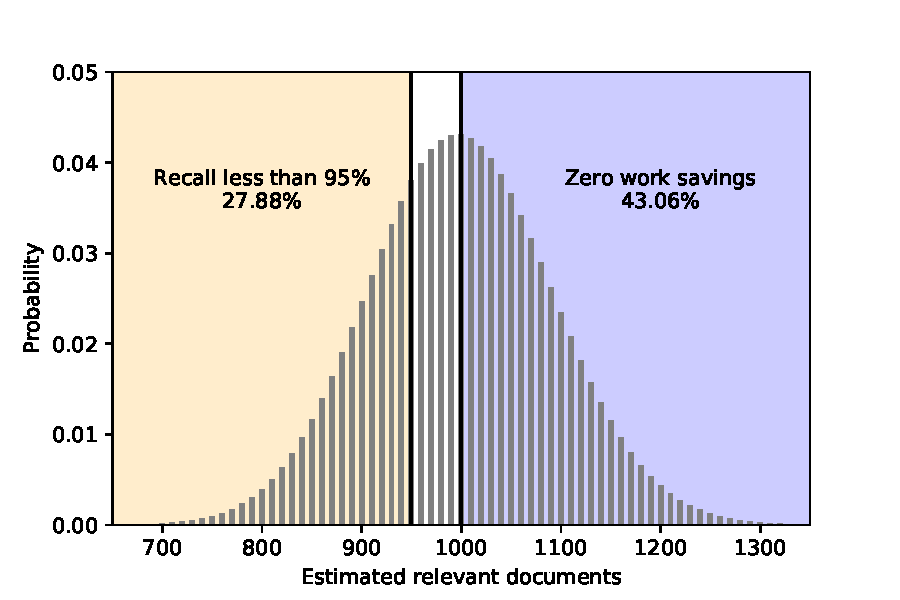
\includegraphics[width=\textwidth]{../images/bir_errors}
%DIFDELCMD < 		%%%
\DIFdelendFL \DIFaddbeginFL 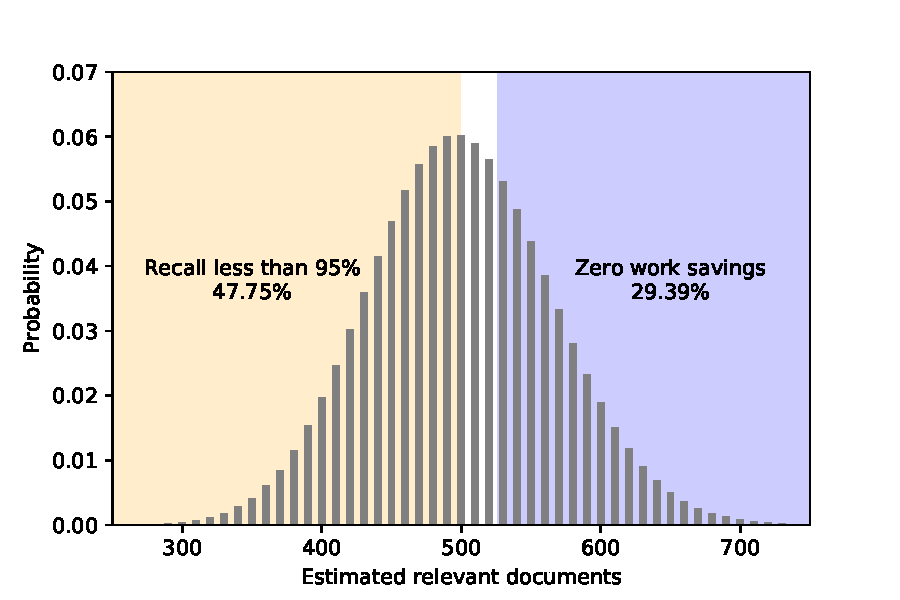
\includegraphics[width=\textwidth]{2_figs_bir_errors.pdf}
			\DIFaddendFL \caption[]%
			{{\small Error types after 1,000 documents \\}}    
			\label{fig:bir_error}
		\end{subfigure}
		\hfill
		\begin{subfigure}[b]{0.475\textwidth}   
			\centering 
			\DIFdelbeginFL %DIFDELCMD < 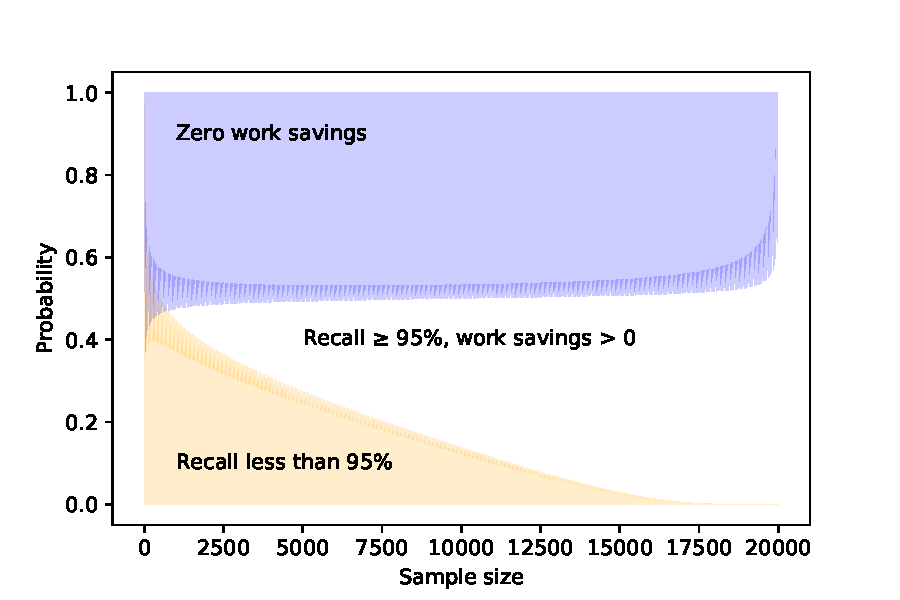
\includegraphics[width=\textwidth]{../images/bir_error_distribution}
%DIFDELCMD < 		%%%
\DIFdelendFL \DIFaddbeginFL 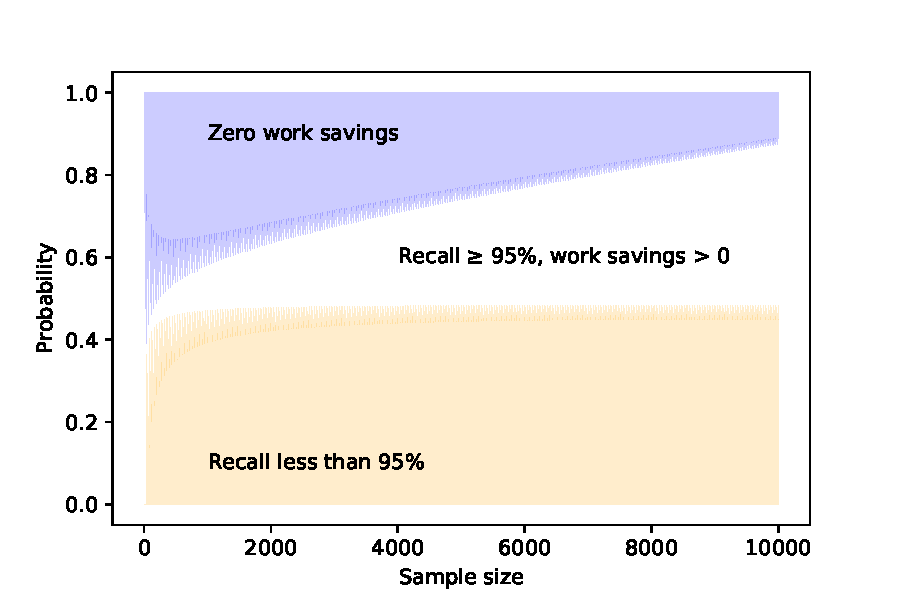
\includegraphics[width=\textwidth]{2_figs_bir_error_distribution.pdf}
			\DIFaddendFL \caption[]%
			{{\footnotesize Error types across sample sizes}}    
			\label{fig:bir_error_distribution}
		\end{subfigure}

		\caption{\small Distribution of under- or over-estimation errors using the BIR sampling method in a dataset of 20,000 documents of which 500 are relevant. Panel (a) shows the probability distribution of the estimated number of relevant documents after a sample of 1,000 documents. Panel (b) shows the probability of each type of error according to the sample size.} 
		\label{bir-sampling}
	\end{figure*}

	\begin{figure}
		\DIFdelbeginFL %DIFDELCMD < 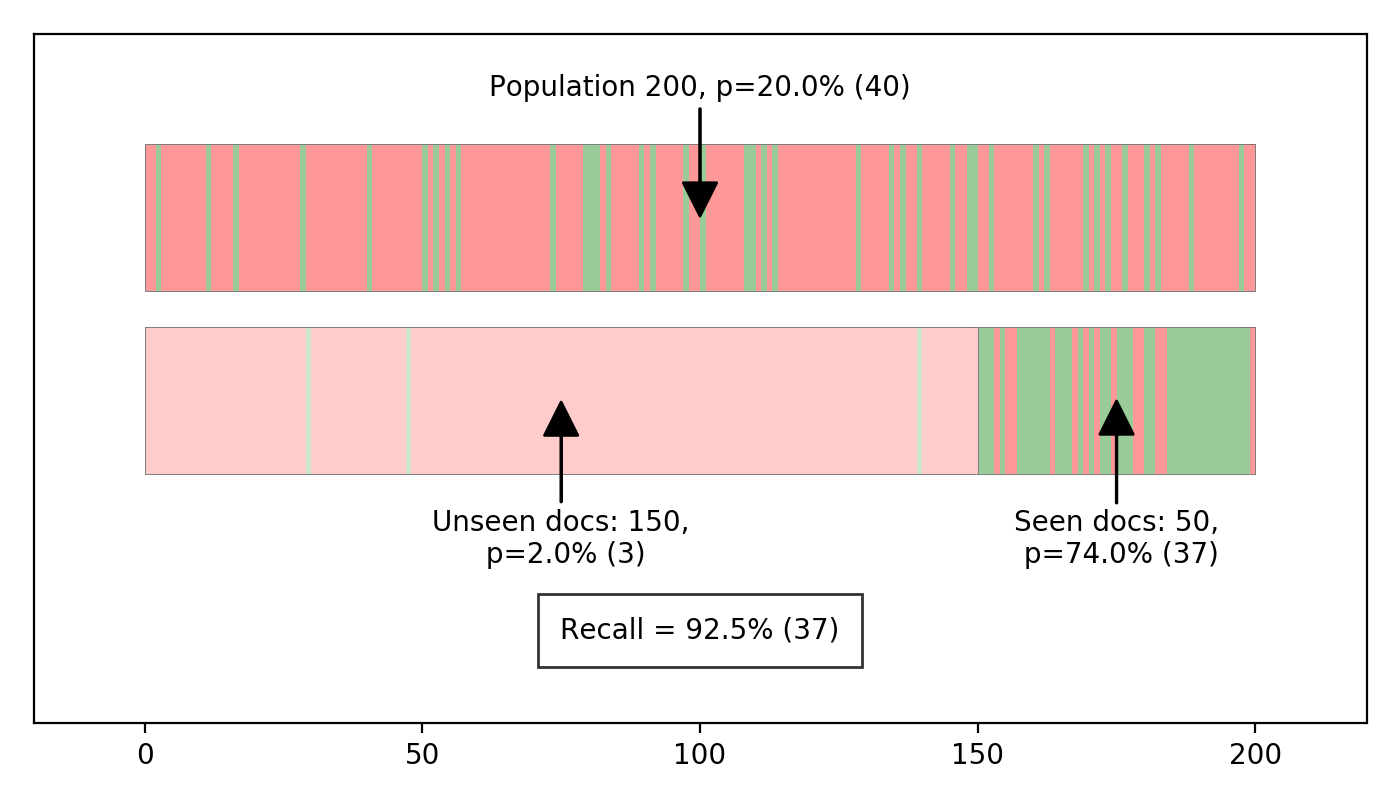
\includegraphics[width=\linewidth]{../images/proportions_1.png}
%DIFDELCMD < 	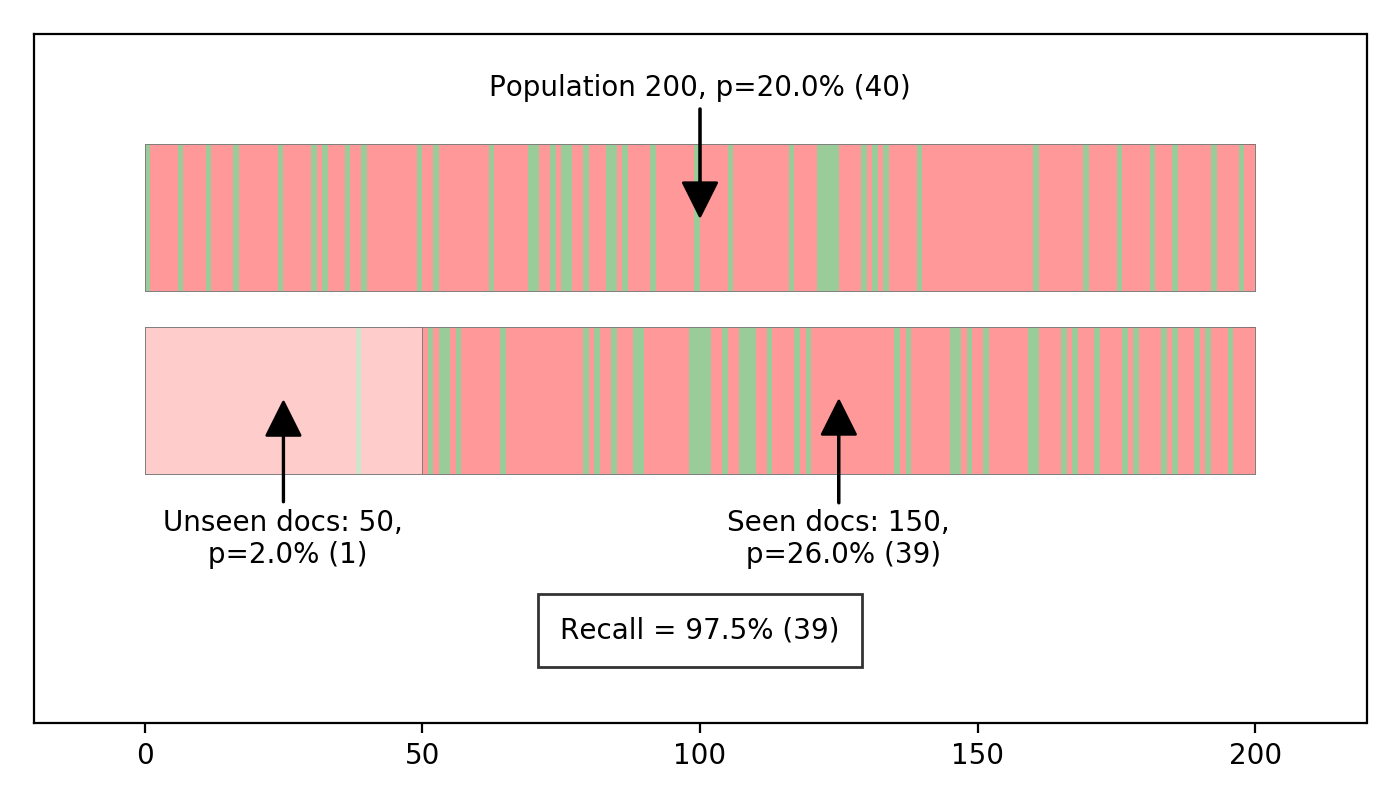
\includegraphics[width=\linewidth]{../images/proportions_2.png}
%DIFDELCMD < 	%%%
\DIFdelendFL \DIFaddbeginFL 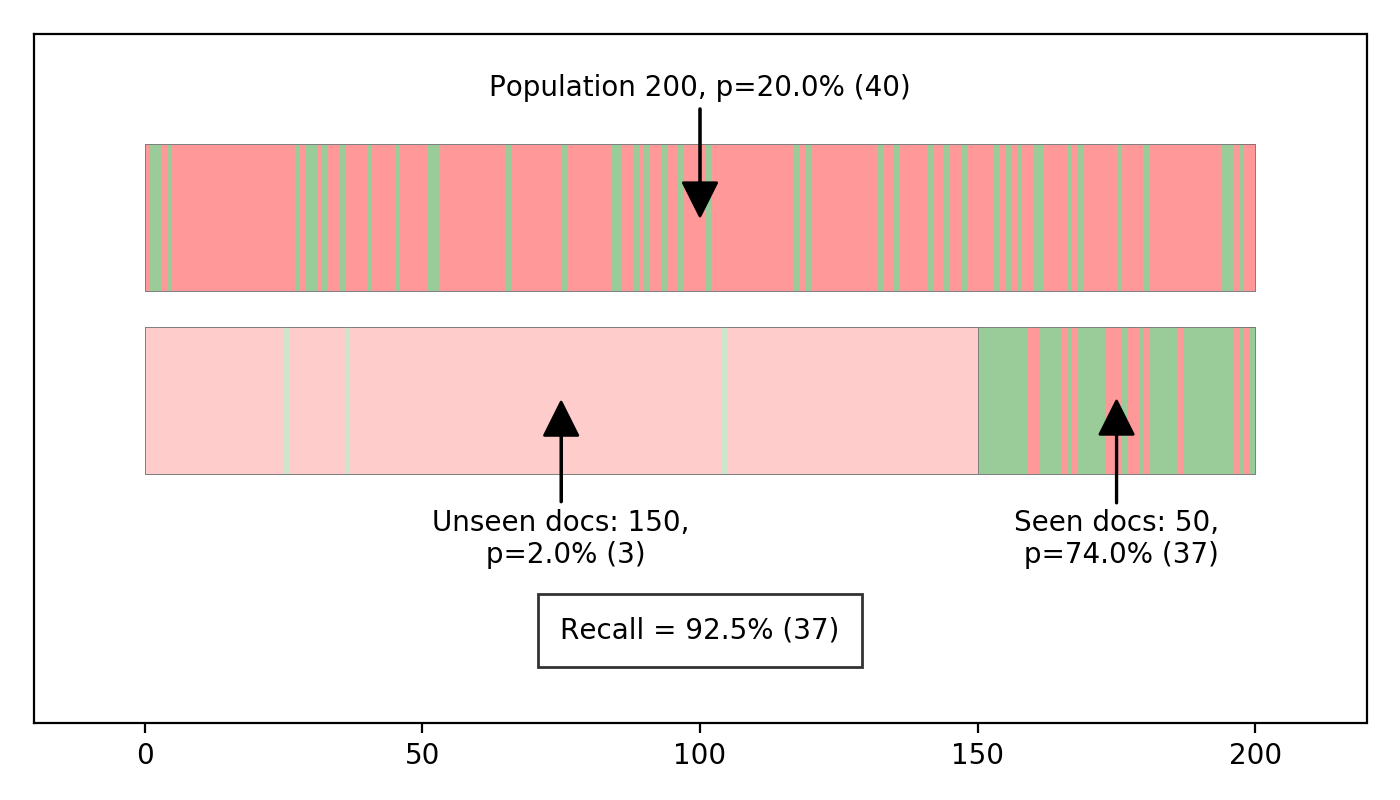
\includegraphics[width=\linewidth]{2_figs_proportions_1.png}
		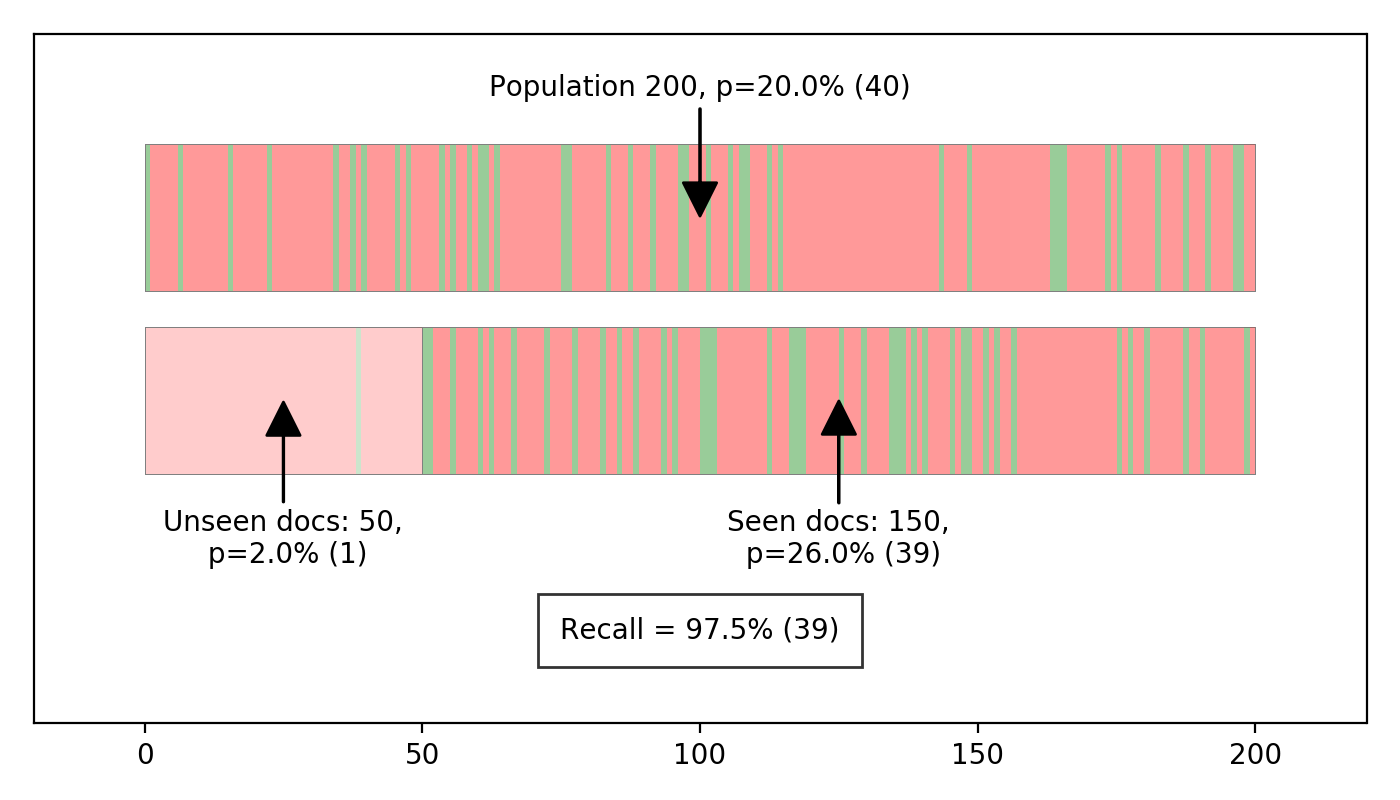
\includegraphics[width=\linewidth]{2_figs_proportions_2.png}
		\DIFaddendFL \caption{Similar low proportions of relevant documents in unseen documents with different consequences for recall. The top bar shows a random distribution of relevant documents (green) and irrelevant documents (red) at a given proportion of relevance. The bottom bar  shows distributions of relevant and irrelevant documents in hypothetical sets of seen (right) and unseen (left - transparent) documents.}
		\label{unseen-proportions}
	\end{figure}

	
	
	\subsubsection*{Heuristic Stopping Criteria}

	Some studies give the example of heuristic stopping criteria based on drawing a given number of irrelevant articles in a row \cite{Jonnalagadda2013, Przybya2018}. 
	We take this as a proxy for estimating that the proportion of documents remaining in the unseen documents is low\DIFaddbegin \DIFadd{, as the probability of observing 0 relevant documents in a given sample (analogous to a set of consecutive irrelevant results) is a decreasing function of the number of relevant documents in the population}\DIFaddend .
	We find this a promising intuition, but argue that 1) it ignores uncertainty, as discussed in relation to the previous method; 
	\DIFdelbegin \DIFdel{and }\DIFdelend 2) it \DIFaddbegin \DIFadd{lacks a formal description that would help to find a suitable threshold for the criterion; and 3) it }\DIFaddend misunderstands the significance of a low proportion of relevant documents in estimating the recall.

	Figure \ref{unseen-proportions} illustrates this \DIFdelbegin \DIFdel{second }\DIFdelend \DIFaddbegin \DIFadd{third }\DIFaddend point. 
	We show two scenarios with identical low proportions of relevant documents observed in the unseen documents.
	In the top figure, machine learning (ML) has performed well, and 74\% of the screened documents were relevant. 
	In the bottom figure, ML has performed less well, and only 26\% of the screened documents were relevant.
	In both cases, only 2\% of unseen documents are relevant, but 2\% of a larger number means more relevant documents are missed.
	Recall is not simply a function of the \DIFdelbegin \DIFdel{relevance of unseen }\DIFdelend \DIFaddbegin \DIFadd{proportion of unseen relevant }\DIFaddend documents, but also of the number of unseen documents. 
	This also means that where ML has performed well (as in the top figure), a low proportion of relevant documents in those not yet checked is indicative of lower recall than where ML has performed less well.
	Likewise, where the proportion of relevant documents in the whole corpus is low, a similarly low proportion of relevant documents is likely to be observed, even when true recall is low. 
	\DIFaddbegin \DIFadd{This shows us that even a perfect estimator of the proportion of unseen relevant documents is insufficient on its own to provide sufficient information about when to stop screening. To estimate recall reliably, it is necessary to take into account the total number of unseen relevant documents (or their proportion times the number of unseen documents).
	}\DIFaddend 

	\subsubsection*{\DIFdelbegin \DIFdel{Other }\DIFdelend \DIFaddbegin \DIFadd{Pragmatic }\DIFaddend stopping criteria}

	Wallace et al. \cite{Wallace2010a} develop a ``simple, operational stopping criterion'': stopping after half the documents have been screened. Although the criterion worked in their experiment, it is unclear how this could be generalised, and its development depended on knowledge of the true relevance values. 
	Jonnalagadda and Petitti \cite{Jonnalagadda2013} note that ``the reviewer can elect to end the process of classifying documents at any point, recognizing that stopping before reviewing all documents involves a trade-off of lower recall for reduced workload'', although clearly the reviewer lacks information about probable recall.
	\DIFaddbegin 

	\subsubsection*{\DIFadd{Novel automatic stopping criteria}}
	\DIFadd{Two examples come from the information retrieval literature. Di Nunzio \cite{DiNunzio2018} presents a novel automatic stopping criterion based on BM25, although recall reported is ``often between 0.92 and 0.94 and consistently over 0.7''.
	}\DIFaddend Yu and Menzies \cite{Yu2019} \DIFdelbegin \DIFdel{adopt a more complicated stopping criterion }\DIFdelend \DIFaddbegin \DIFadd{also present a stopping criterion based on BM25 }\DIFaddend which allows the user to target a specific level of recall. 
	However, reviewers are not given the opportunity to specify a confidence level, and for two of the four datasets in which they tested their criteria, the median achieved recall at a stopping criteria targeting 95\% recall was below 95\%. \DIFdelbegin \DIFdel{Di Nunzio \cite{DiNunzio2018} also present an innovative stopping criteria, but it does not take into account uncertainty, and produces results }\DIFdelend \DIFaddbegin \DIFadd{In each case, the reliability of the estimate is dependent on the performance of the model.
	}

	\DIFadd{Finally, Howard et al. \cite{Howard2020} present a method to estimate recall based on the number of irrelevant documents $D$ observed in a list of documents since the $\delta th$ previous relevant document. 
	They reason that this should follow the negative binomial distribution based on the proportion of remaining relevant documents $p$, and use this information to estimate $\hat{p}$, and with this, the total number of relevant articles and the estimated recall.
	}

	\DIFadd{However, their method does not quantify uncertainty, but can only claim that the method ``}\DIFaddend \textit{\DIFdelbegin \DIFdel{near}%DIFDELCMD < } %%%
\DIFdel{a target recallthreshold, rather than above it in a reliable proportion of cases. 
}\DIFdelend \DIFaddbegin \DIFadd{tends}} \DIFadd{to result in a conservative estimate of recall'' (emphasis ours). This is not guaranteed by the criterion itself but rather a finding of the simulation with example datasets. Further the authors do not give sufficient information to reproduce their results, providing neither code (they describe their own proprietary software), nor an equation for $\hat{p}$. Additionally, the criterion requires a tuning parameter $\delta$, which users may have insufficient information to set optimally.
	Lastly, because screening is a form of sampling without replacement, the negative hypergeometric distribution should be preferred to the negative binomial, even though the latter can be a good approximation for cases with large numbers of documents.
	}

	\DIFaddend These last examples are promising developments, but \DIFaddbegin \DIFadd{they all }\DIFaddend fail to take into account the needs of live systematic reviews, where the reliability of and ease of communication about recall are paramount\DIFaddbegin \DIFadd{, and the results are independent of model performance. In the following, we explain our own method, which provides clearly communicable estimates of recall, which manage uncertainty in a way robust to model performance}\DIFaddend .

	\subsection*{Methods}

	\subsection*{A Statistical Stopping Criterion for Active Learning}

	\DIFdelbegin \subsubsection*{\DIFdel{Random Sampling}}
	%DIFAUXCMD
\DIFdelend \DIFaddbegin \DIFadd{In our screening setup, we start off with $N_{tot}$ documents that are potentially relevant. $\rho_{tot}$ of these documents are actually relevant, but we don't know this value \textit{a priori}. As we screen relevant documents we include them, so $\rho_{seen}$ represents the number of relevant documents screened, and recall $\tau$ is given by 
	}\DIFaddend 

	\DIFdelbegin \DIFdel{After using machine learning to select which documents are screened by humans as described above, we begin }\DIFdelend \DIFaddbegin \begin{equation}
	\DIFadd{\tau = \frac{\rho_{seen}}{\rho_{tot}}
	\label{eq:recall-def}
	}\end{equation}

	\DIFadd{We set a target recall $\tau_{tar}$ and a confidence level $\alpha$. 
	We want to keep screening until $\tau \geq \tau_{tar}$, and devise a hypothesis test to estimate whether this is the case with a given level of confidence. 
	We do this	based on interrupting the active-learning process and }\DIFaddend drawing a random sample from the remaining \DIFdelbegin \DIFdel{documents (when this happens is described below)}\DIFdelend \DIFaddbegin \DIFadd{unseen documents. 
	We first describe this test, before showing how a variation on the test can be used to decide when to begin drawing a random sample. 
	}

	\subsubsection*{\DIFadd{Random Sampling}}

	\DIFadd{At the start of the sample, $N_{AL}$ is the number of documents seen during the active learning process, and $N$ is the number of documents remaining, so that 
	}

	\begin{equation}
	\DIFadd{N = N_{tot} - N_{AL}
	}\end{equation} 

	\DIFadd{We refer to the number  of relevant documents seen during active learning as $\rho_{AL}$, and the number of remaining relevant documents as $K$. We do not know the value of $K$ but know that it is given by the total number of relevant documents minus the number of relevant documents seen during active learning}\DIFaddend .

	\DIFdelbegin \DIFdel{We use random sampling to estimate the probability that a target recall $\tau$ has been achieved. }\DIFdelend \DIFaddbegin \begin{equation}
	\DIFadd{K = \rho_{tot} - \rho_{AL}
	\label{eq:K}
	}\end{equation}

	\DIFadd{We now take random draws from the remaining $N$ documents, and denote the number of documents drawn with $n$ and the number of relevant documents drawn with $k$. The number of relevant documents seen is updated by adding the number of relevant documents seen since sampling began to the number of relevant documents seen during active learning.
	}

	\begin{equation}
	\DIFadd{\rho_{seen} = \rho_{AL} + k
	\label{eq:rho_seen}
	}\end{equation}

	\DIFadd{We proceed to form a null hypothesis that the true value of recall is less than our target recall:
	}

	\begin{equation}
	\DIFadd{H_0 : \tau < \tau_{tar}
	\label{eq:null_hypothesis}
	}\end{equation}

	\DIFaddend Because we are sampling \DIFdelbegin \DIFdel{a binary outcome }\DIFdelend without replacement, we can use the hypergeometric distribution to \DIFdelbegin \DIFdel{formulate a statistical test. The hypergeometric distribution tells us }\DIFdelend \DIFaddbegin \DIFadd{find out }\DIFaddend the probability of observing $k$ relevant documents in \DIFaddbegin \DIFadd{a sample of }\DIFaddend $n$ \DIFdelbegin \DIFdel{draws from a finite }\DIFdelend \DIFaddbegin \DIFadd{documents from a }\DIFaddend population of $N$ documents \DIFdelbegin \DIFdel{with }\DIFdelend \DIFaddbegin \DIFadd{of which }\DIFaddend $K$ \DIFdelbegin \DIFdel{relevant documents. }\DIFdelend \DIFaddbegin \DIFadd{are relevant. We know that $k$ is distributed hypergeometrically:
	}\DIFaddend 

	\begin{equation}
	k \sim Hypergeometric(N, K, n)
	\end{equation}
	\DIFdelbegin %DIFDELCMD < 

%DIFDELCMD < 	%%%
\DIFdel{In our case, we know $k$, $n$ and $N$ after each draw, but $K$ is unknown. We therefore substitute }\DIFdelend \DIFaddbegin 

	\DIFadd{We introduce }\DIFaddend a hypothetical value \DIFdelbegin \DIFdel{$\hat{K}$: }\DIFdelend \DIFaddbegin \DIFadd{for $K$, which we call $K_{tar}$. This represents }\DIFaddend the minimum number of relevant documents \DIFdelbegin \DIFdel{in the sample had the recall target been missed}\DIFdelend \DIFaddbegin \DIFadd{remaining at the start of sampling compatible with our null hypothesis that recall is below our target}\DIFaddend .

	\DIFdelbegin \DIFdel{Recall $R$ is given by the number of relevant documents that have been seen $\rho_{s}$ over the number of relevant documents in the whole dataset $\rho_{tot}$
	}%DIFDELCMD < 

%DIFDELCMD < 	%%%
\begin{displaymath}
		\DIFdel{R = \frac{\rho_{seen}}{\rho_{tot}}
	}\end{displaymath}
	%DIFAUXCMD
\DIFdelend \DIFaddbegin \begin{equation}
	\DIFadd{K_{tar} = \lfloor \frac{\rho_{seen}}{\tau_{tar}}-\rho_{AL}+1 \rfloor
	}\end{equation}
	\DIFaddend 

	\DIFdelbegin \DIFdel{The }\DIFdelend \DIFaddbegin \DIFadd{This equation is derived by combining Eqs.~\ref{eq:recall-def} and \ref{eq:rho_seen}. Because $k$ can only take integer values, $K_{tar}$ is the smallest integer that satisfies the inequality in Eq.~\ref{eq:null_hypothesis}.
	With $K_{tar}$, we can reformulate our null hypothesis: the true }\DIFaddend number of relevant documents in the \DIFdelbegin \DIFdel{whole dataset is the sum of $\hat{\rho}$ relevant documents seen before random sampling began and $\tilde{K}$ relevant documents unseen at the start of random sampling.
	We can therefore express $R$ as
	}\DIFdelend \DIFaddbegin \DIFadd{sample is greater than our hypothetical value.
	}\DIFaddend 

	\begin{equation}
	\DIFdelbegin \DIFdel{R = \frac{\dot{\rho}}{\hat{\rho} + \tilde{K}},
	}\DIFdelend \DIFaddbegin \DIFadd{H_0 : K > K_{tar}
	}\DIFaddend \end{equation}

	\DIFdelbegin \DIFdel{Substituting the target recall $\tau$ for $R$, reorganising and rounding up to the next integer, we can, after each draw, calculate $\hat{K}$, which is the minimum number of relevant documents that could have been remaining when random sampling started, if recall were lower than the target}\DIFdelend \DIFaddbegin \DIFadd{We test this by calculating the probability of observing $k$ or fewer relevant documents from the hypergeometric distribution given by $K_{tar}$, using the cumulative probability mass function}\DIFaddend .

	\begin{equation}
	\DIFdelbegin %DIFDELCMD < \hat{K} %%%
\DIFdelend \DIFaddbegin \DIFadd{p }\DIFaddend = \DIFdelbegin %DIFDELCMD < \lceil %%%
\DIFdel{\frac{\rho}{\tau} - }%DIFDELCMD < \hat{\rho} \rceil
%DIFDELCMD < 	%%%
\DIFdelend \DIFaddbegin \DIFadd{P(X \leq k)$, where $X \sim Hypergeometric(N,K_{tar},n)
	}\label{eq:p-value}
	\DIFaddend \end{equation}

	\DIFdelbegin \DIFdel{We use the cumulative distribution function of the hypergeometric distribution to estimate the probability $p$ of having observed }\DIFdelend \DIFaddbegin \DIFadd{Because the cumulative probability mass function $P(X \leq k)$ is decreasing with increasing $K$, this gives the maximum probability of observing }\DIFaddend $k$ \DIFdelbegin \DIFdel{or fewer relevant documents in the sample given $\hat{K}$. This function gives us an upper bound on the probability of observing no more than the number of relevant documents in our random sample that we did, if our recall target had not been achieved.
	If this is below our confidence level $1 - \alpha$}\DIFdelend \DIFaddbegin \DIFadd{for all values of $K$ compatible with our null hypothesis. Similar arguments have been made to derive confidence intervals for estimating the parameter $K$ in the hypergeometric distribution function \citep{Buonaccorsi1987, Sahai1995} and the derivation of an equivalent criterion could use the upper limit of such a confidence interval of an estimated $K$ from the observation of $k$.
	}

	\DIFadd{We can reject our null hypothesis and stop screening if the maximum probability of obtaining our observed results given our null hypothesis $p$ is below $1-\alpha$. This means}\DIFaddend , we can \DIFdelbegin \DIFdel{reject the null hypothesis that the recall target was not achieved}\DIFdelend \DIFaddbegin \DIFadd{report the likelihood that we achieve a recall above our target as being more than $\alpha$ }\footnote{\DIFadd{The notebook, }\url{https://github.com/mcallaghan/rapid-screening/blob/master/analysis/hyper_criteria_theory.ipynb}\DIFadd{, in the github repository accompanying this paper contains a step by step explanation of this method with code and examples}}\DIFaddend .

	
	
	\subsubsection*{\DIFdelbegin \DIFdel{Pseudo-random sampling}\DIFdelend \DIFaddbegin \DIFadd{Ranked quasi-sampling}\DIFaddend }

	\DIFdelbegin \DIFdel{In }\DIFdelend \DIFaddbegin \DIFadd{We now proceed to describe a special case of the method described above which we (1) use as a heuristic in }\DIFaddend order to decide when to begin \DIFdelbegin \DIFdel{a random sample, we employ pseudo-random sampling, where we treat previously screened documents as a random sample. The distribution of relevant documents among }\DIFdelend \DIFaddbegin \DIFadd{random sampling; and (2) test as an independent stopping criterion. The method works by treating batches of }\DIFaddend previously screened documents \DIFdelbegin \DIFdel{is clearly not random , as documents predicted to be relevant are prioritised. It is reasonable to assume, though, that the density of relevant documents is greater among previously screeneddocuments than among remaining unseen documents. This would make the following estimates conservative.
	}\DIFdelend \DIFaddbegin \DIFadd{as if they were random samples.
	}\DIFaddend 

	\DIFdelbegin \DIFdel{After reviewing each document, $S$ documents have been screened,
	and $U$ documents are yet to be seen. We treat $i = 1 \dots S$ of the previously screened documents as a random sample}\DIFdelend \DIFaddbegin \DIFadd{We calculate $p$ as above for subsets of the already screened documents. Concretely, we use subsets of documents $A_i$ by looking back to the last $i$ documents, $A_i = \{d_{N_{seen} - 1}, ..., d_{N_{seen} - i}\}$, where the documents $d$ are indexed in the order in which they have been screened. For a specific $i$, this corresponds to  random sampling beginning after seeing $i$ documents in the section above.
	Thus, we set 
	$N_{AL}$ to $i$, 
	$n$ to $N_{seen}-i$, 
	$\rho_{AL}$ to the number of relevant documents seen when $i$ documents had been seen,
	and $k$ to the number of relevant documents seen since $i$ documents had been seen}\DIFaddend , and calculate $p$ \DIFdelbegin \DIFdel{, using the method above, for each sample, taking the minimum across all samples $p_{min}$. If $p_{min}$ is less than $1-\frac{\alpha}{2}$, we }\DIFdelend \DIFaddbegin \DIFadd{according to Eq.~\ref{eq:p-value}.
	We compute $p$ for all sets $A_i$ with $i \in {N_{seen}-1 \dots 1}$.
	This gives us a vector $\bm{p}$, representing the values of $p$ which would have been estimated at each point at which we could have stopped active learning and began random sampling. The lowest probability of our null hypothesis being true that we would have thereby obtained is given by $p_{min}$. With the vectorized implementation included in our accompanying code, these calculations are completed in less than the time it would take a human to code the next document.
	}

	\DIFadd{First, we use this method as a useful heuristic for deciding when to stop active learning, and }\DIFaddend switch to random sampling. \DIFdelbegin \DIFdel{We also calculate $p_{min}$ for the remaining documents as if we had not switched to random sampling and record the recall and work saved when }\DIFdelend \DIFaddbegin \DIFadd{For this, we choose a higher threshold for the likelihood, $p_{min} < 1-\frac{\alpha}{2}$. Second, we use the same ranked quasi-sampling as an independent stopping criterion, by continuing screening with active learning until }\DIFaddend $p_{min} < 1 - \alpha$. We present \DIFdelbegin \DIFdel{these in the results below as }\DIFdelend the \DIFdelbegin \DIFdel{psuedo-random sampling criterion }\DIFdelend \DIFaddbegin \DIFadd{results of this second procedure separately below.
	}

	\DIFadd{Given that the documents seen during active learning are ranked according to predicted relevance, they do not in fact represent a random sample. This means that the test is unlikely to be accurate. It would be reasonable to assume that the proportion of relevant documents in each ranked quasi-sample is as high if not higher than the proportion of relevant documents in the unseen documents. This assumption would make this estimator conservative. As such it works in a similar way to the criterion proposed by Howard et al. \cite{Howard2020}, although it makes use of more information and provides hypothesis testing rather than just a point estimate of recall}\DIFaddend .

	
	\medskip

	\begin{figure}
		\DIFdelbeginFL %DIFDELCMD < 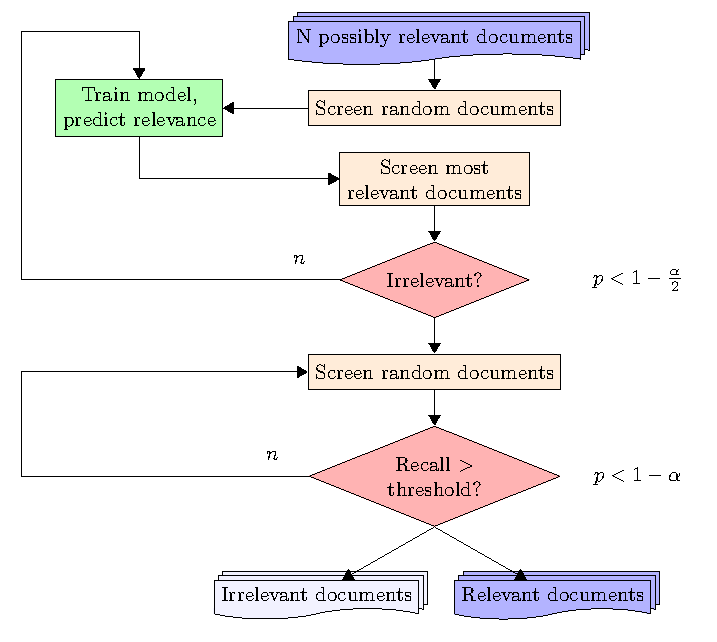
\includegraphics[width=0.7\linewidth]{../images/flow}
%DIFDELCMD < 		%%%
\DIFdelendFL \DIFaddbeginFL 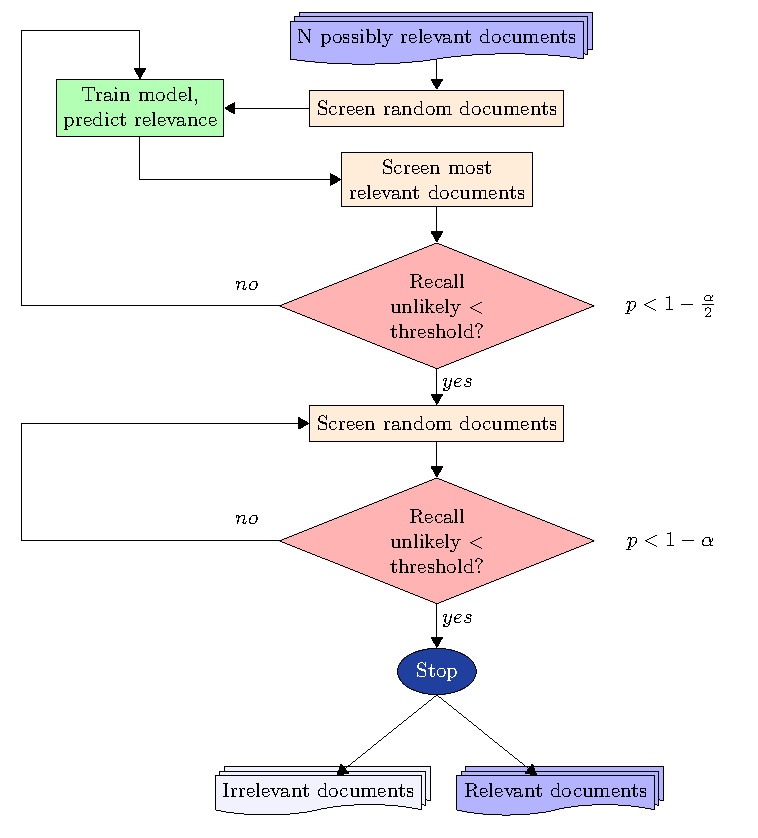
\includegraphics[width=0.7\linewidth]{2_figs_flow.pdf}
		\DIFaddendFL \caption{A workflow for active learning in screening with a statistical stopping criterion}
		\label{flow}
	\end{figure}

	\subsection*{Evaluation}

	We evaluate each of the criteria discussed on real world test data, operationalising the heuristic stopping criteria with 50, 100, and 200 consecutive irrelevant records. We run 100 iterations on each dataset and record the following measures.
	\begin{itemize}
		\item \textbf{Actual Recall}: The recall when the stopping criteria was met
		\item \textbf{WS-SC}: Work saved when the stopping criteria was met
		\item \textbf{Additional Burden}: the work saved when the criterion was triggered subtracted from the work saved when the recall target was actually achieved.

	\end{itemize}
	For simplicity, we use a basic SVM model \cite{Cortes95, Pedregosa2011}, with 1-2 word n-grams taken from the document abstracts used as input data. We start with random samples of 200 documents (we do not employ Shemilt et al's methods for identifying the ``optimal'' sample size, as we showed these in the methods section to be unhelpful). Subsequently, we ``screen'', that is, we reveal the labels of, batches of the 20 documents with the highest predicted relevance scores, retraining the model after each batch. \DIFaddbegin \DIFadd{Theoretically, using smaller batch sizes could mean that the recall target is achieved more quickly, but this is a trade-off between computational time spent training, and the speed at which the algorithm can ``learn''. However this is a modelling choice which may affect work saved, but not recall. }\DIFaddend Each criterion is evaluated after each document is ``screened''.
	For our criteria, we set the target recall value to 95\% and the confidence level to 95\%.

	
	%\subsubsection*{Evaluation Data}
	\begin{table}
		\DIFdelbeginFL %DIFDELCMD < \begin{tabular}{lllrrr}
\toprule
{} &                  dataset & data\_source &     N &  r\_docs &    p \\
\midrule
0  &      UrinaryIncontinence &       cohen &   284 &      68 & 0.24 \\
1  &           Antihistamines &       cohen &   287 &      90 & 0.31 \\
2  &                Estrogens &       cohen &   349 &      79 & 0.23 \\
3  &                   NSAIDS &       cohen &   358 &      83 & 0.23 \\
4  &        OralHypoglycemics &       cohen &   475 &     135 & 0.28 \\
5  &                 Triptans &       cohen &   594 &     205 & 0.35 \\
6  &                     ADHD &       cohen &   803 &      83 & 0.10 \\
7  &   AtypicalAntipsychotics &       cohen &  1030 &     333 & 0.32 \\
8  &   CalciumChannelBlockers &       cohen &  1103 &     257 & 0.23 \\
9  &     ProtonPumpInhibitors &       cohen &  1210 &     227 & 0.19 \\
10 &  SkeletalMuscleRelaxants &       cohen &  1348 &      30 & 0.02 \\
11 &                     COPD &     copd\_pb &  1443 &     179 & 0.12 \\
12 &               Kitchenham &    fastread &  1700 &      45 & 0.03 \\
13 &                   Opiods &       cohen &  1769 &      43 & 0.02 \\
14 &             BetaBlockers &       cohen &  1872 &     270 & 0.14 \\
15 &            ACEInhibitors &       cohen &  2234 &     168 & 0.08 \\
16 &                  Statins &       cohen &  2743 &     152 & 0.06 \\
17 &               ProtonBeam &     copd\_pb &  4108 &     240 & 0.06 \\
18 &               Radjenovic &    fastread &  5999 &      47 & 0.01 \\
19 &                   Wahono &    fastread &  7002 &      62 & 0.01 \\
20 &                     Hall &    fastread &  8911 &     104 & 0.01 \\
\bottomrule
\end{tabular}

%DIFDELCMD < 		%%%
\DIFdelendFL \DIFaddbeginFL \begin{tabular}{lllrrr}
\toprule
{} &                  dataset & data\_source &     N &  r\_docs &    p \\
\midrule
0  &      UrinaryIncontinence &       cohen &   284 &      68 & 0.24 \\
1  &           Antihistamines &       cohen &   287 &      90 & 0.31 \\
2  &                Estrogens &       cohen &   349 &      79 & 0.23 \\
3  &                   NSAIDS &       cohen &   358 &      83 & 0.23 \\
4  &        OralHypoglycemics &       cohen &   475 &     135 & 0.28 \\
5  &                 Triptans &       cohen &   594 &     205 & 0.35 \\
6  &                     ADHD &       cohen &   803 &      83 & 0.10 \\
7  &   AtypicalAntipsychotics &       cohen &  1030 &     333 & 0.32 \\
8  &   CalciumChannelBlockers &       cohen &  1103 &     257 & 0.23 \\
9  &     ProtonPumpInhibitors &       cohen &  1210 &     227 & 0.19 \\
10 &  SkeletalMuscleRelaxants &       cohen &  1348 &      30 & 0.02 \\
11 &                     COPD &     copd\_pb &  1443 &     179 & 0.12 \\
12 &               Kitchenham &    fastread &  1700 &      45 & 0.03 \\
13 &                   Opiods &       cohen &  1769 &      43 & 0.02 \\
14 &             BetaBlockers &       cohen &  1872 &     270 & 0.14 \\
15 &            ACEInhibitors &       cohen &  2234 &     168 & 0.08 \\
16 &                  Statins &       cohen &  2743 &     152 & 0.06 \\
17 &               ProtonBeam &     copd\_pb &  4108 &     240 & 0.06 \\
18 &               Radjenovic &    fastread &  5999 &      47 & 0.01 \\
19 &                   Wahono &    fastread &  7002 &      62 & 0.01 \\
20 &                     Hall &    fastread &  8911 &     104 & 0.01 \\
\bottomrule
\end{tabular}

		\DIFaddendFL \caption{Dataset properties}
		\label{tab:data}
	\end{table}

	The systematic review datasets used for testing are described in table \ref{tab:data}. We use the seminal collection of systematic reviews used to develop machine learning applications for document screening by Aaron Cohen and co-authors in 2006 \cite{Cohen2006}, along with the widely used Proton Beam \cite{Terasawa2009} and COPD \cite{Castaldi2009} datasets, and computer science datasets used to test FASTREAD \cite{Yu2019}. Testing on datasets with different properties and from different domains is key to establishing criteria appropriate for general use. Choosing as broad as possible data also prevents us from being able to ``tune'' our machine learning approach in ways that may work well for specific datasets but not generalise well. Work savings, even maximum work savings are therefore below the state of the art recorded for each of these datasets. In this way we can show how well the criteria perform even when the model performs badly.

	%As a last step, we explain the factors that increase or decrease the performance of our criteria, using a simple regression model.

	All computational steps required to reproduce this analysis are documented online at \url{https://github.com/mcallaghan/rapid-screening}.

	\section*{Results}

	Figure \ref{recall-wss} shows the actual recall and work savings achieved when each stopping criteria has been satisfied. 
	For comparison, we also include the results that would have been achieved with \textit{a priori} knowledge of the data, that is, the work saved when the 95\% recall target was actually reached. In a live systematic review, reviewers would never know when this had been reached, but these are the work savings most often reported in machine learning for systematic review screening studies.

	
	\begin{figure*}
		\centering
		\begin{subfigure}[b]{0.475\textwidth}   
			\centering 
			\DIFdelbeginFL %DIFDELCMD < 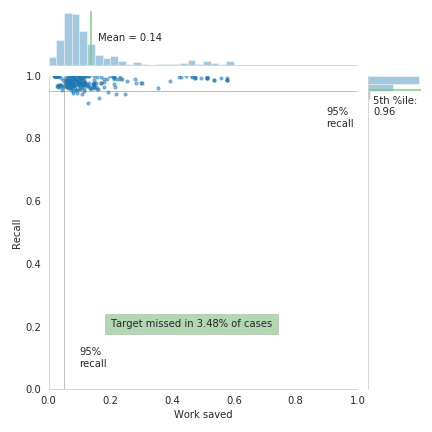
\includegraphics[width=\textwidth]{../images/jointplot_hyper}
%DIFDELCMD < 		%%%
\DIFdelendFL \DIFaddbeginFL 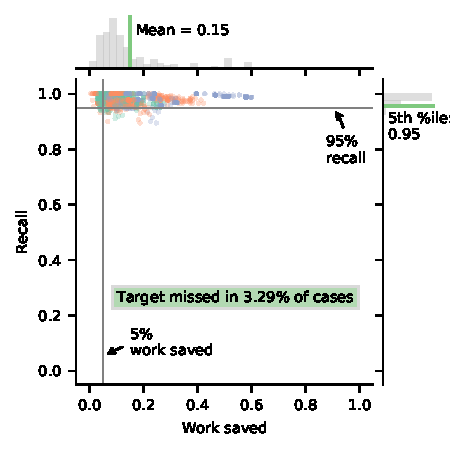
\includegraphics[width=\textwidth]{2_figs_jointplot_hyper.pdf}
			\DIFaddendFL \caption[]%
			{{\small Hypergeometric sampling \\}}    
			\label{fig:hyper}
		\end{subfigure}
		\hfill
		\begin{subfigure}[b]{0.475\textwidth}   
			\centering 
			\DIFdelbeginFL %DIFDELCMD < 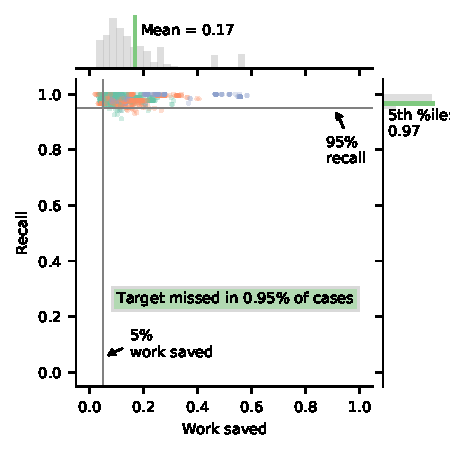
\includegraphics[width=\textwidth]{../images/jointplot_nrs}
%DIFDELCMD < 		%%%
\DIFdelendFL \DIFaddbeginFL 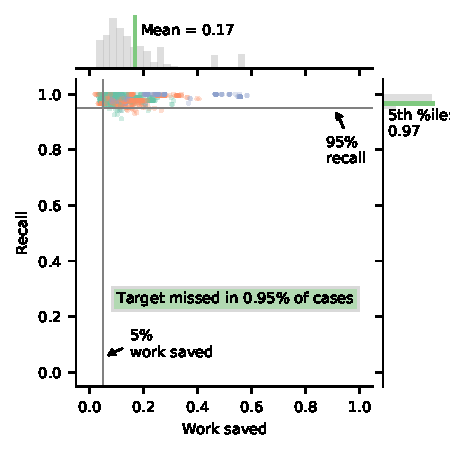
\includegraphics[width=\textwidth]{2_figs_jointplot_nrs.pdf}
			\DIFaddendFL \caption[]%
			{{\footnotesize \DIFdelbeginFL \DIFdelFL{Pseudorandom hypergeometric sampling}\DIFdelendFL \DIFaddbeginFL \DIFaddFL{Ranked quasi-sampling}\DIFaddendFL }}    
			\label{fig:nrs}
		\end{subfigure}
		\vskip\baselineskip
		\begin{subfigure}[b]{0.475\textwidth}
			\centering
			\DIFdelbeginFL %DIFDELCMD < 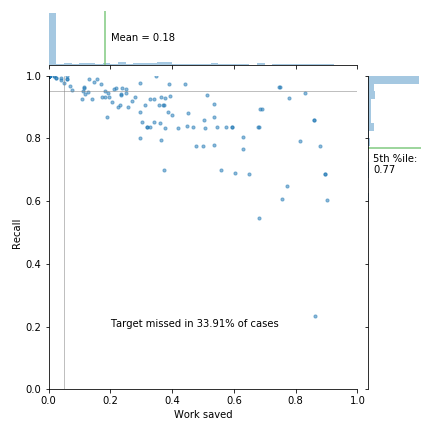
\includegraphics[width=\textwidth]{../images/jointplot_bir}
%DIFDELCMD < 		%%%
\DIFdelendFL \DIFaddbeginFL 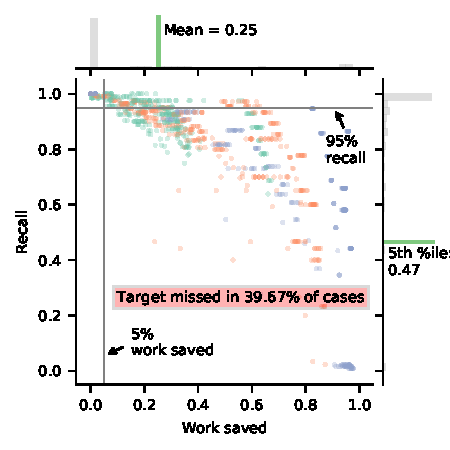
\includegraphics[width=\textwidth]{2_figs_jointplot_bir.pdf}
			\DIFaddendFL \caption[Network2]%Example-Image
			{{\small Baseline Sampling}}    
			\label{fig:bir}
		\end{subfigure}
		\hfill
		\begin{subfigure}[b]{0.475\textwidth}  
			\centering 
			\DIFdelbeginFL %DIFDELCMD < 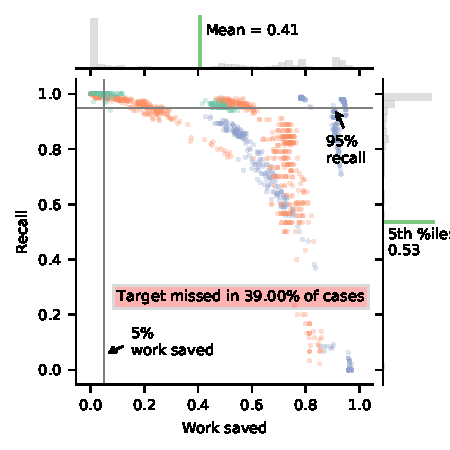
\includegraphics[width=\textwidth]{../images/jointplot_ih_50}
%DIFDELCMD < 		%%%
\DIFdelendFL \DIFaddbeginFL 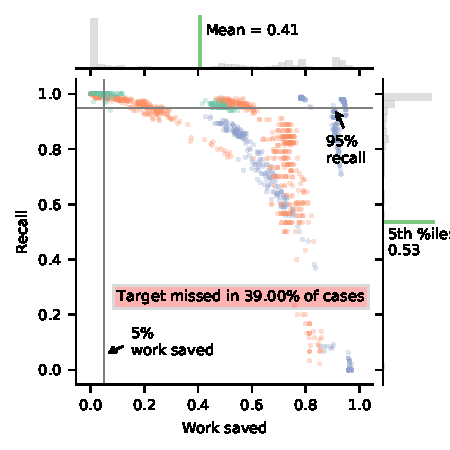
\includegraphics[width=\textwidth]{2_figs_jointplot_ih_50.pdf}
			\DIFaddendFL \caption[]%
			{{\small 50 consecutive irrelevant results}}    
			\label{fig:ih_50}
		\end{subfigure}
		\vskip\baselineskip
		\begin{subfigure}[b]{0.475\textwidth}   
			\centering 
			\DIFdelbeginFL %DIFDELCMD < 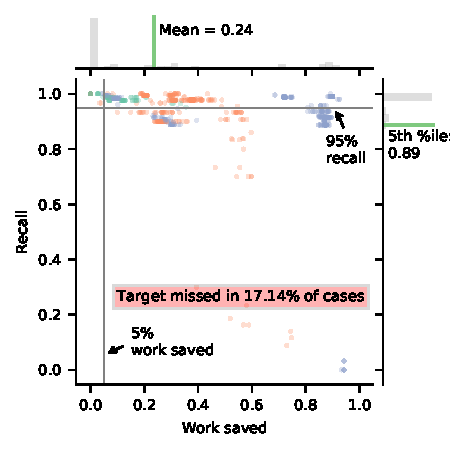
\includegraphics[width=\textwidth]{../images/jointplot_ih_200}
%DIFDELCMD < 		%%%
\DIFdelendFL \DIFaddbeginFL 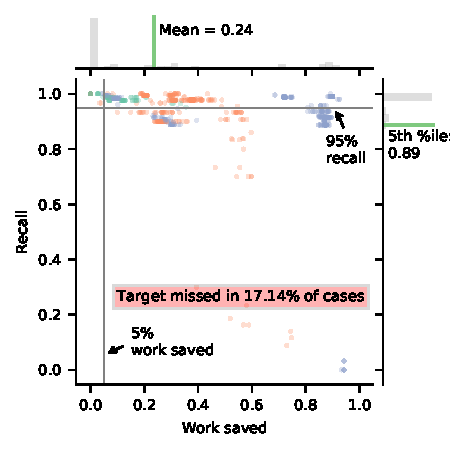
\includegraphics[width=\textwidth]{2_figs_jointplot_ih_200.pdf}
			\DIFaddendFL \caption[]%
			{{\small 200 consecutive irrelevant results \\}}    
			\label{fig:ih_200}
		\end{subfigure}
		\hfill
		\begin{subfigure}[b]{0.475\textwidth}   
			\centering 
			\DIFdelbeginFL %DIFDELCMD < 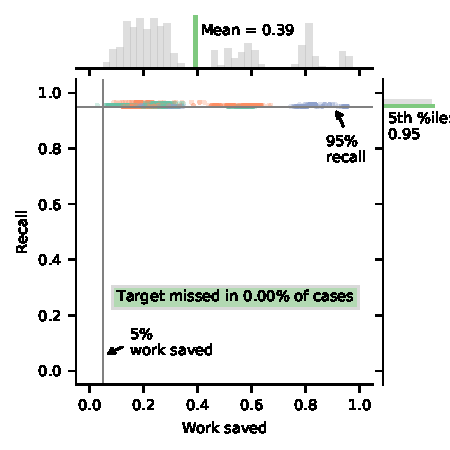
\includegraphics[width=\textwidth]{../images/jointplot_pf.pdf}
%DIFDELCMD < 		%%%
\DIFdelendFL \DIFaddbeginFL 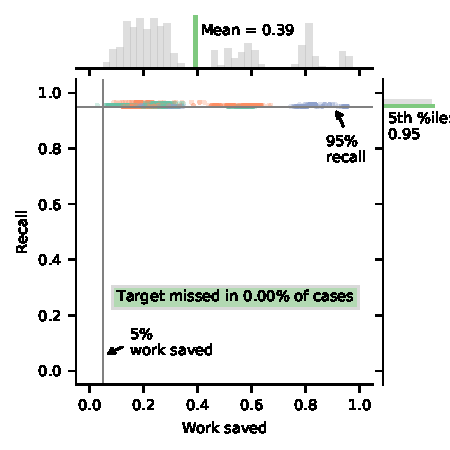
\includegraphics[width=\textwidth]{2_figs_jointplot_pf.pdf}
			\DIFaddendFL \caption[]%
			{{\footnotesize \textit{a priori} knowledge}}   
			\label{fig:pf}
		\end{subfigure}

		\caption{\small Distribution of recall and work saved after each stopping criteria. Green dots show results for datasets with less than 1,000 documents, orange dots show datasets with 1,000 - 2,000 documents, and blue dots show datasets with more than 2,000 documents.} 
		\label{recall-wss}
	\end{figure*}

	\begin{figure*}
		\centering
		\begin{subfigure}[b]{0.475\textwidth}   
			\centering 
			\DIFdelbeginFL %DIFDELCMD < 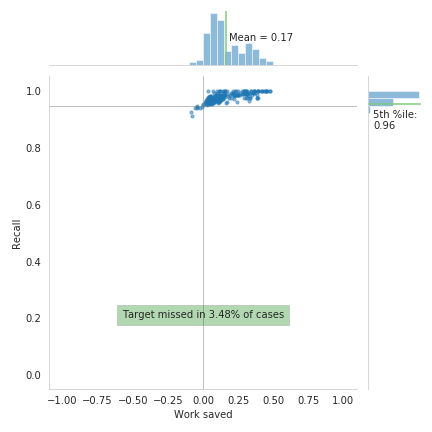
\includegraphics[width=\textwidth]{../images/jointplot_burden_hyper}
%DIFDELCMD < 		%%%
\DIFdelendFL \DIFaddbeginFL 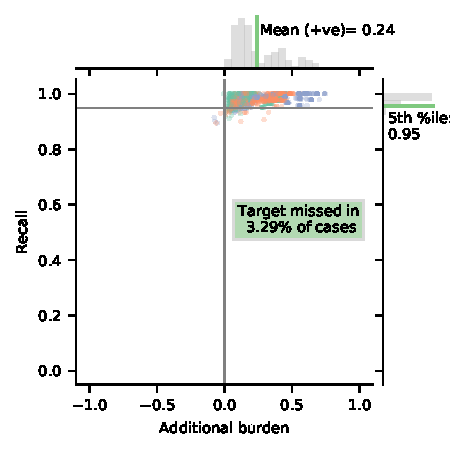
\includegraphics[width=\textwidth]{2_figs_jointplot_burden_hyper.pdf}
			\DIFaddendFL \caption[]%
			{{\small Hypergeometric sampling \\}}    
			\label{fig:hyper_ab}
		\end{subfigure}
		\hfill
		\begin{subfigure}[b]{0.475\textwidth}   
			\centering 
			\DIFdelbeginFL %DIFDELCMD < 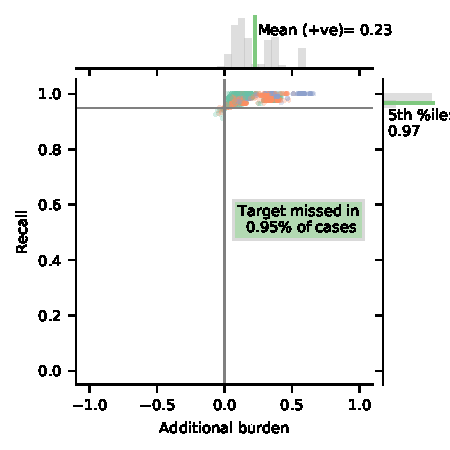
\includegraphics[width=\textwidth]{../images/jointplot_burden_nrs.pdf}
%DIFDELCMD < 		%%%
\DIFdelendFL \DIFaddbeginFL 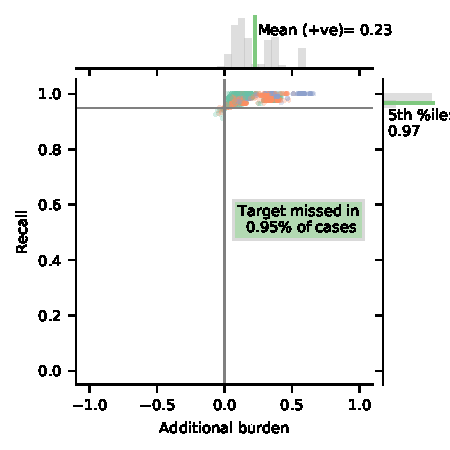
\includegraphics[width=\textwidth]{2_figs_jointplot_burden_nrs.pdf}
			\DIFaddendFL \caption[]%
			{{\footnotesize \DIFdelbeginFL \DIFdelFL{Pseudorandom hypergeometric sampling}\DIFdelendFL \DIFaddbeginFL \DIFaddFL{Ranked quasi-sampling}\DIFaddendFL }}    
			\label{fig:nrs_ab}
		\end{subfigure}
		\hfill
		\vskip\baselineskip
		\begin{subfigure}[b]{0.475\textwidth}
			\centering
			\DIFdelbeginFL %DIFDELCMD < 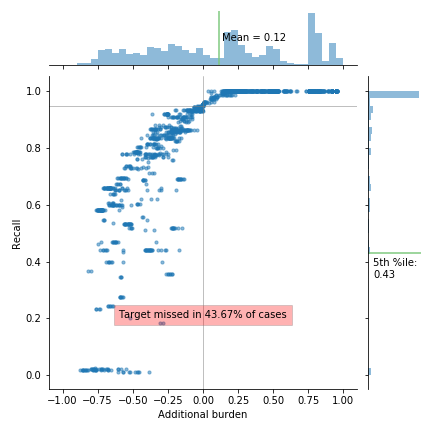
\includegraphics[width=\textwidth]{../images/jointplot_burden_bir}
%DIFDELCMD < 		%%%
\DIFdelendFL \DIFaddbeginFL 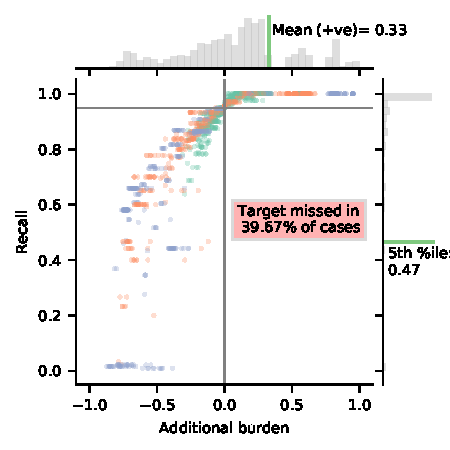
\includegraphics[width=\textwidth]{2_figs_jointplot_burden_bir.pdf}
			\DIFaddendFL \caption[Network2]%Example-Image
			{{\small Baseline Sampling}}    
			\label{fig:bir_ab}
		\end{subfigure}
		\hfill
		\begin{subfigure}[b]{0.475\textwidth}  
			\centering 
			\DIFdelbeginFL %DIFDELCMD < 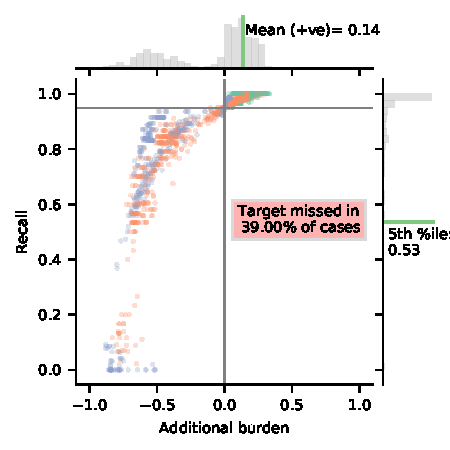
\includegraphics[width=\textwidth]{../images/jointplot_burden_ih_50}
%DIFDELCMD < 		%%%
\DIFdelendFL \DIFaddbeginFL 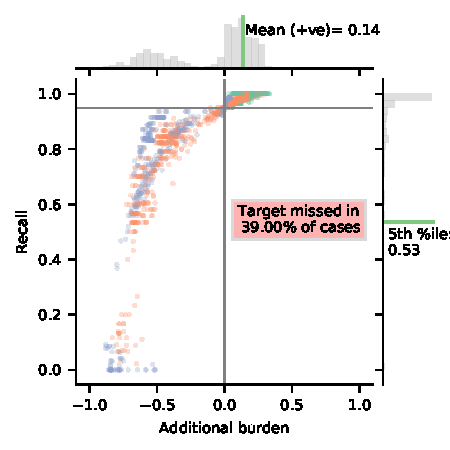
\includegraphics[width=\textwidth]{2_figs_jointplot_burden_ih_50.pdf}
			\DIFaddendFL \caption[]%
			{{\small 50 consecutive irrelevant results}}    
			\label{fig:ih_50_ab}
		\end{subfigure}
		\vskip\baselineskip

		\begin{subfigure}[b]{0.475\textwidth}   
			\centering 
			\DIFdelbeginFL %DIFDELCMD < 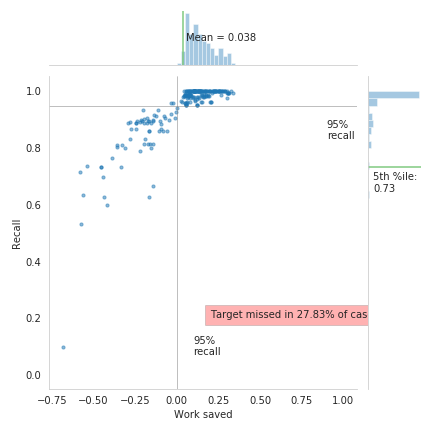
\includegraphics[width=\textwidth]{../images/jointplot_burden_ih_100}
%DIFDELCMD < 		%%%
\DIFdelendFL \DIFaddbeginFL 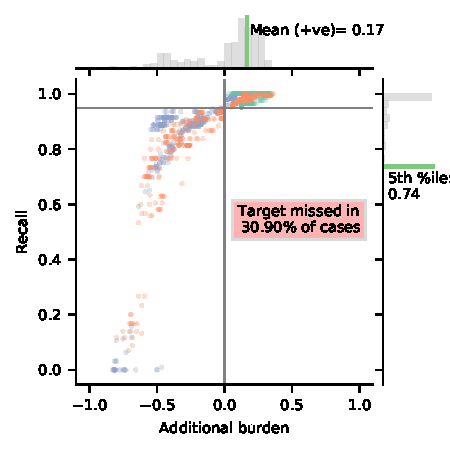
\includegraphics[width=\textwidth]{2_figs_jointplot_burden_ih_100.pdf}
			\DIFaddendFL \caption[]%
			{{\small 100 consecutive irrelevant results }}    
			\label{fig:ih_200_ab}		

		\end{subfigure}
		\hfill
		\begin{subfigure}[b]{0.475\textwidth}   
			\centering 
			\DIFdelbeginFL %DIFDELCMD < 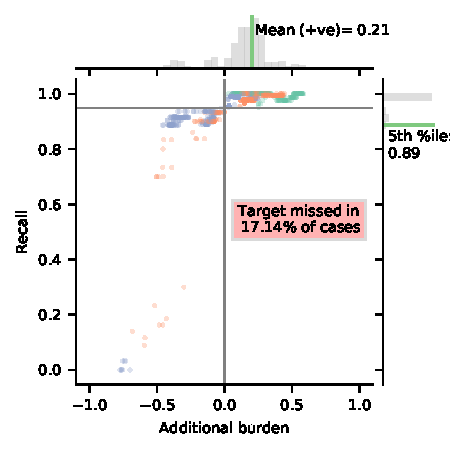
\includegraphics[width=\textwidth]{../images/jointplot_burden_ih_200.pdf}
%DIFDELCMD < 		%%%
\DIFdelendFL \DIFaddbeginFL 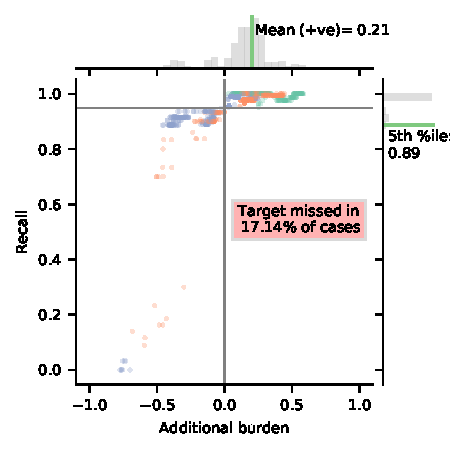
\includegraphics[width=\textwidth]{2_figs_jointplot_burden_ih_200.pdf}
			\DIFaddendFL \caption[]%
			{{\footnotesize 200 consecutive irrelevant results }}    
			\label{fig:ih_100_ab}
		\end{subfigure}

		\caption{\small Distribution of recall and additional burden after each stopping criterion. Additional burden is the work saved when the criterion was triggered minus the work saved when the target was reached. Coloring of data points as in Fig. \ref{recall-wss}.}
		\label{recall-burden}
	\end{figure*}

	
	
	Both the random sampling and the \DIFdelbegin \DIFdel{pseudorandom }\DIFdelend \DIFaddbegin \DIFadd{ranked }\DIFaddend sampling criteria achieve the target threshold of 95\% in more than 95\% of cases. 
	\DIFdelbegin \DIFdel{In fact , the pseudorandom sampling }\DIFdelend \DIFaddbegin \DIFadd{That this is greater than 95\% is accounted for by the fact that random sampling sometimes begins after the target has been achieved, in which case the null hypothesis would be \text{a priori} impossible.
	The ranked quasi-sampling }\DIFaddend criterion  outperforms the random sampling criterion with respect to both recall and work savings, saving a mean of 17\% of the work compared to 15\%, and missing the target in only 0.95\% compared to 3.29\% of cases. In theory, the \DIFdelbegin \DIFdel{pseudorandom }\DIFdelend \DIFaddbegin \DIFadd{ranked }\DIFaddend sampling criteria is conservative if the assumption holds that documents chosen by machine learning are not less likely to be relevant than those chosen at random. Based on our experiments, this assumption seems reasonable, and accounts for the higher recall. Because the \DIFdelbegin \DIFdel{pseudorandom sampling }\DIFdelend \DIFaddbegin \DIFadd{ranked quasi-sampling }\DIFaddend criterion can flexibly choose its sample, whereas the random criterion has to wait for a random sample to be triggered, the criterion is also triggered earlier, as it can make use of more data. This accounts for the higher work savings.

	
	
	The baseline sampling criteria (Figure \ref{fig:bir}) misses the 95\% recall target in 39.67\% of cases, while the most common work saving is 0\%. This is in line with our expectations that, due to random sampling error, the expected number of documents will often be over-estimated or under-estimated, resulting in zero work savings or poor recall.

	The Heuristic stopping criteria, both for 50 consecutive irrelevant results (Figure \ref{fig:ih_50} - IH50), and for 200 irrelevant results (Figure \ref{fig:ih_200}) also perform unreliably. Although the mean work saved for IH50 is 41\%, the target is missed in 39\% of cases. The cases below the horizontal grey line indicate instances where work has been saved at the expense of achieving the recall target.

	\begin{figure}
		\DIFdelbeginFL %DIFDELCMD < 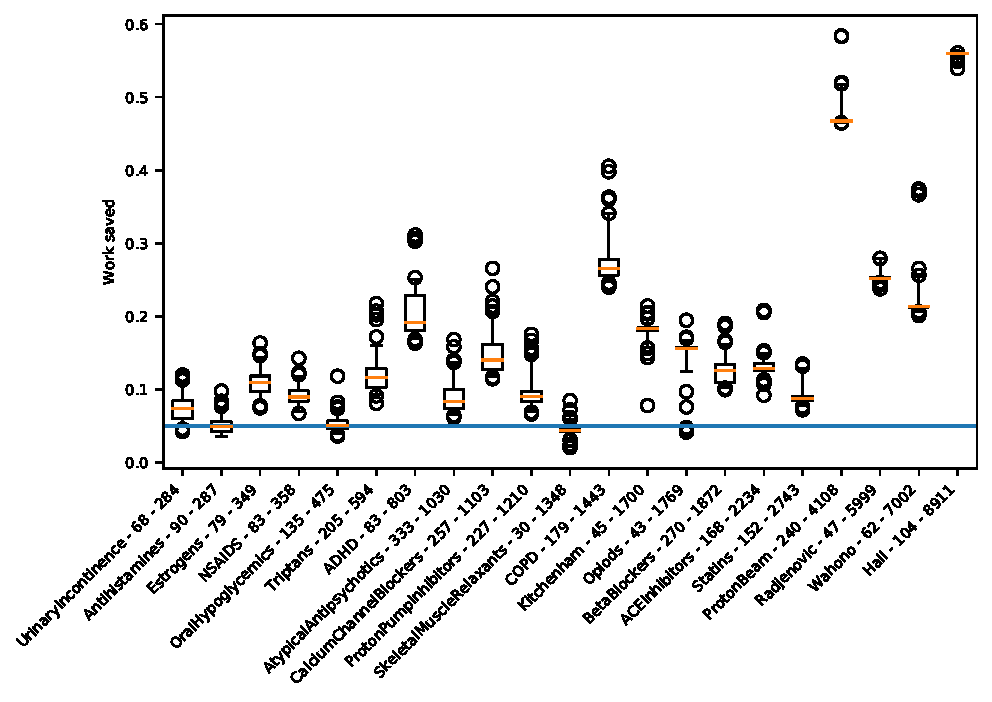
\includegraphics[width=0.9\linewidth]{../images/wss_nrs}
%DIFDELCMD < 		%%%
\DIFdelendFL \DIFaddbeginFL 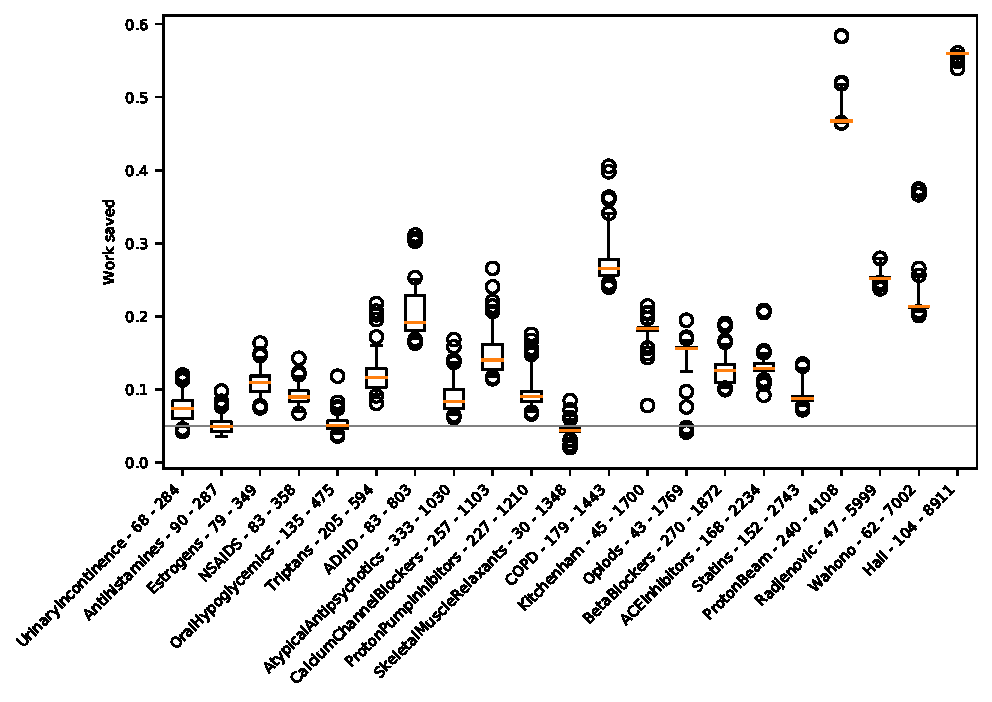
\includegraphics[width=0.9\linewidth]{2_figs_wss_nrs.pdf}
		\DIFaddendFL \caption{Work saved for the \DIFdelbeginFL \DIFdelFL{pseudorandom sampling }\DIFdelendFL \DIFaddbeginFL \DIFaddFL{ranked quasi-sampling }\DIFaddendFL method in each dataset. Labels show the number of relevant documents and the total number of documents. The datasets are presented in order of the number of documents. The whiskers represent the 5th and 95th percentiles. The grey line shows work savings of 5\%. }
		\label{wss}
	\end{figure}

	\begin{figure*}
		\centering
		\begin{subfigure}[b]{0.475\textwidth}
			\centering
			\DIFdelbeginFL %DIFDELCMD < 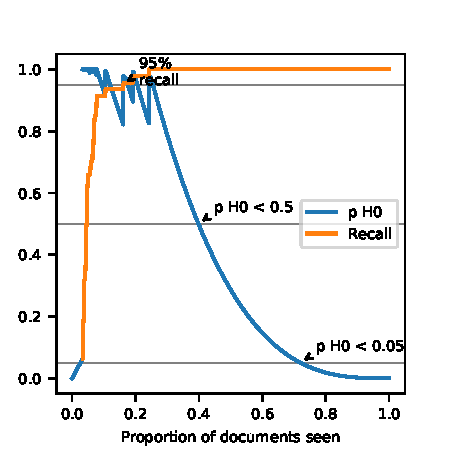
\includegraphics[width=\textwidth]{../images/h0_paths_Radjenovic.pdf}
%DIFDELCMD < 			%%%
\DIFdelendFL \DIFaddbeginFL 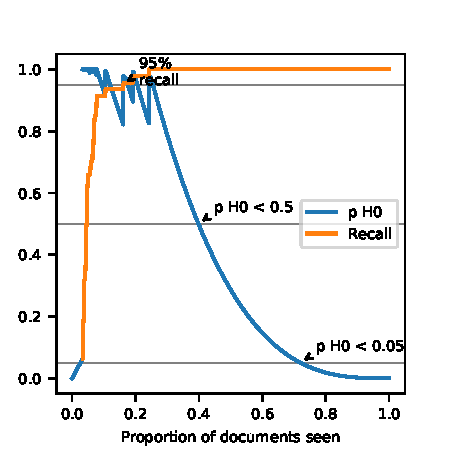
\includegraphics[width=\textwidth]{2_figs_h0_paths_Radjenovic.pdf}
			\DIFaddendFL \caption[Network2]%Example-Image
			{{\small Radjenovic}}    
			\label{fig:Radjenovic}
		\end{subfigure}
		\hfill
		\begin{subfigure}[b]{0.475\textwidth}  
			\centering 
			\DIFdelbeginFL %DIFDELCMD < 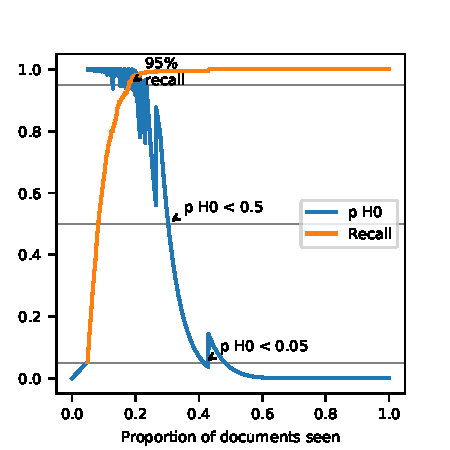
\includegraphics[width=\textwidth]{../images/h0_paths_ProtonBeam.pdf}
%DIFDELCMD < 			%%%
\DIFdelendFL \DIFaddbeginFL 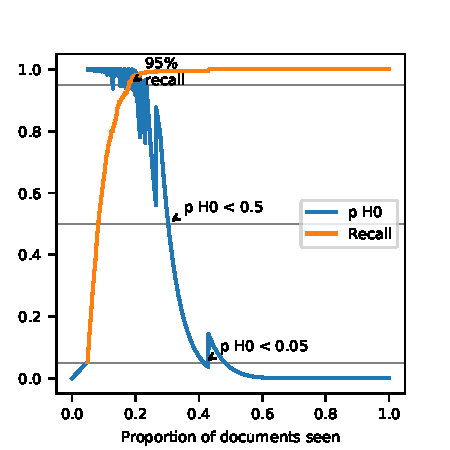
\includegraphics[width=\textwidth]{2_figs_h0_paths_ProtonBeam.pdf}
			\DIFaddendFL \caption[]%
			{{\small ProtonBeam}}    
			\label{fig:ProtonBeam}
		\end{subfigure}
		\vskip\baselineskip
		\begin{subfigure}[b]{0.475\textwidth}
			\centering
			\DIFdelbeginFL %DIFDELCMD < 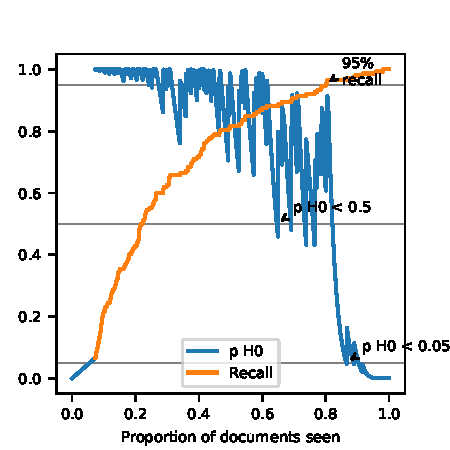
\includegraphics[width=\textwidth]{../images/h0_paths_Statins.pdf}
%DIFDELCMD < 			%%%
\DIFdelendFL \DIFaddbeginFL 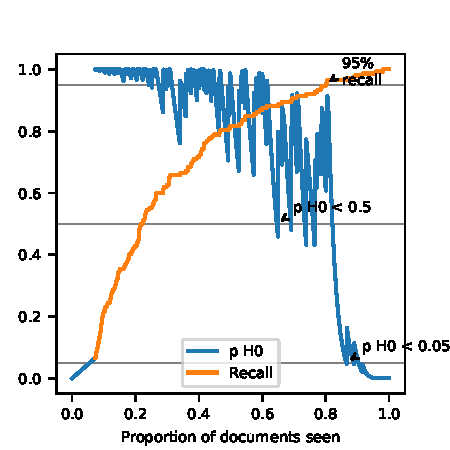
\includegraphics[width=\textwidth]{2_figs_h0_paths_Statins.pdf}
			\DIFaddendFL \caption[Network2]%Example-Image
			{{\small Statins}}    
			\label{fig:Statins}
		\end{subfigure}
		\hfill
		\begin{subfigure}[b]{0.475\textwidth}  
			\centering 
			\DIFdelbeginFL %DIFDELCMD < 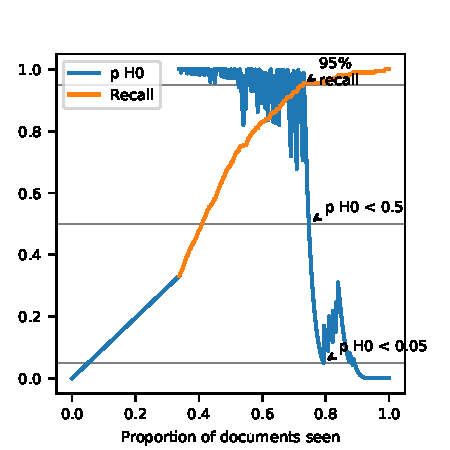
\includegraphics[width=\textwidth]{../images/h0_paths_Triptans.pdf}
%DIFDELCMD < 			%%%
\DIFdelendFL \DIFaddbeginFL 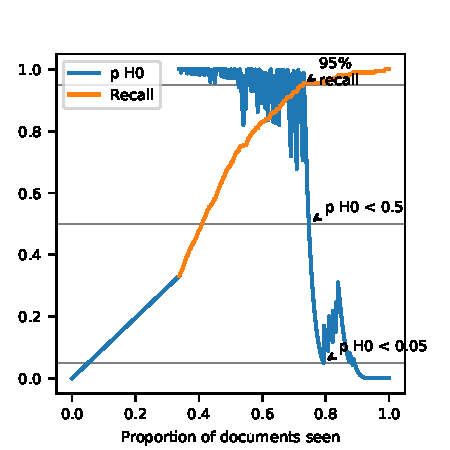
\includegraphics[width=\textwidth]{2_figs_h0_paths_Triptans.pdf}
			\DIFaddendFL \caption[]%
			{{\small Triptans}}    
			\label{fig:Triptans}
		\end{subfigure}

		\caption{\small The path of recall (yellow) and the p-value of H0 for four different datasets} 
		\label{H0paths}
	\end{figure*}

	In figure \ref{recall-burden} we rescale the x axis, calling it additional burden, which is simply the work saved when the criterion is triggered minus the work saved when the recall target was actually achieved. This measure indicates whether the stopping criterion was triggered too early (negative values), or too late (positive values). The figure directly highlights the tradeoffs involved in deciding when to stop screening: For our criteria, there is mostly a small additional burden which comes with the necessity to make sure the desired recall target has been reached and reject the null hypothesis that this has not been the case. For the other criteria, there are many cases in which additional burden is negative, i.e. the criterion has been triggered too early. In these cases, however, the desired recall is hardly ever reached.

	To help explain the different work savings that were observed in our experiments, we show the distribution of work savings from our \DIFdelbegin \DIFdel{pseudorandom }\DIFdelend \DIFaddbegin \DIFadd{ranked quasi-sampling }\DIFaddend criterion for each dataset in figure \ref{wss}. In general, higher work savings are possible when the total number of documents is larger. However, in datasets with a low proportion of relevant documents, many documents need to be screened to achieve a high confidence that there are only few relevant documents remaining in the unseen ones. Therefore, smaller work savings are possible. 

	Figure \ref{H0paths} shows the recall and the probability of the null hypothesis for the best performing iteration of four datasets. Although the 95\% recall target is achieved very quickly in the Radjenovic dataset, the null hypothesis cannot be excluded until much later. This is because the dataset has only 47 relevant documents out of a population of 5,999. After the 95\% recall target was achieved, 45 out of 47 relevant documents had been seen and 5,029 documents remained. The null hypothesis was therefore that 3 or more of these 5,029 documents were relevant, which requires a lot of evidence to disprove. The burden of proof was smaller in the case of the Proton Beam dataset: at the point that the 95\% recall threshold was reached, the null hypothesis to disprove was that a minimum of 13 out of 3,369 remaining documents were relevant. 

	The Statins and Triptans datasets show how the criterion performs when the machine learning model has performed poorly in predicting relevant results. In each case, 95\% recall is achieved with close to 20\% of documents remaining. With fewer documents remaining, it takes fewer screening decisions to rule out the possibility that the number of relevant documents left is incompatible with the achievement of the recall target.

	\section*{Discussion}

	Our results show that it is possible to use machine learning to achieve a given level of recall with a given level of confidence. The tradeoff for achieving recall reliably is that the work saving achieved is less than the maximum possible work saving. However, for large datasets with a significant proportion of relevant documents, the additional effort required to satisfy the criterion will be small compared to the work saved by using machine learning. This makes the approach well suited to broad topics with lots of literature. In other words, it is precisely where machine learning will be most useful that the additional effort will be small.

	Different use cases for machine learning enhanced screening may also carry different requirements for recall, or different tolerances for uncertainty. These can be flexibly accommodated within our stopping criterion. Importantly, the ability to make probabilistic statements about the chance of achieving a given recall target makes it possible to clearly communicate the implications of using machine learning enhanced screening to readers and reviewers who are not machine learning specialists. This is extremely important in live systematic reviews.

	Our criteria have the further advantage that they are independent of the choice or performance of the machine learning model. If a model performs badly at discerning relevant from irrelevant results, the only consequence will be that the work saved will be low. With other criteria this may result in poor recall. 
	When using machine learning for screening, poor recall can result in biased results, while low work savings represent no loss to the reviewer as compared to not using machine learning.

	\DIFaddbegin \DIFadd{One caveat in the derivation of our criteria is that we did not address the potential problem of multiple testing formally. Such a derivation is mathematically challenging and beyond the scope of this paper. However, the performance of the criteria shows that this is of limited practical concern. Formally describing screening procedures with iterative testing should be a next step towards even more rigorous stopping criteria and should be fully worked out in future research.
	}

	\DIFaddend So far, systematic review standards have no way of accommodating screening with machine learning. 
	We hope that the reliability and clarity of reporting offered by our stopping criteria make them suitable for incorporation into standards, so that machine learning for systematic review screening can fulfil its promise of reducing workload and making more ambitious reviews tractable.

	\section*{Conclusion}

	This paper demonstrates the \DIFdelbegin \DIFdel{unsuitability }\DIFdelend \DIFaddbegin \DIFadd{drawbacks }\DIFaddend of existing stopping criteria for machine learning approaches to document screening, \DIFdelbegin \DIFdel{and proposes }\DIFdelend \DIFaddbegin \DIFadd{particularly with regard to reliability. We propose }\DIFaddend a simple method that delivers reliable recall, independent of machine learning approach or model performance. Our robust statistical stopping criteria allow users to easily communicate the implications of their use of machine learning, making machine learning enhanced screening ready for live reviews.

	
	\begin{backmatter}

		\DIFaddbegin \section*{\DIFadd{Ethics approval}}
		\DIFadd{Not applicable.
		}

		\section*{\DIFadd{Consent for publication}}
		\DIFadd{Not applicable.
		}

		\section*{\DIFadd{Availability of data and materials}} 
		\DIFadd{All computational steps required to reproduce this analysis are documented online at }\url{https://github.com/mcallaghan/rapid-screening}\DIFadd{.
		}

		\DIFaddend \section*{Competing interests}
		The authors declare that they have no competing interests.

		\section*{Author's contributions}
		MC designed the research and conducted the experiments. FMH contributed to the development of the statistical basis for the stopping criterion. Both authors wrote and edited the manuscript.

		\section*{Acknowledgements}
		Max Callaghan is supported by a PhD scholarship from the Heinrich Böll Foundation. Finn M\"{u}ller-Hansen acknowledges funding from the German Federal Ministry of Research and Education within the Strategic Scenario Analysis (START) project (grant reference: 03EK3046B).

		\DIFdelbegin %DIFDELCMD < \bibliography{mendeley}
%DIFDELCMD < 	%%%
\DIFdelend \DIFaddbegin \bibliography{3_bib_mendeley}
		\DIFaddend \bibliographystyle{vancouver}

	\end{backmatter}
\end{document}